\section*{Problema 4: Una clave y un secreto en AES }

En este ejercicio se aplican técnicas de criptoanalisis para recuperar una clave secreta de 50 caracteres oculta en un texto con ruido. En particular, las acciones a realizar consisten en procesar un archivo de texto (\texttt{file.txt}) mediante reglas especificas basadas en números primos y desplazamientos alfabéticos para construir la clave. Posteriormente, esta clave debe validarse en un listado de hashes SHA-256 y utilizarse para abrir un mensaje cifrado mediante el algoritmo moderno AES-GCM (Advanced Encryption Standard - Galois/Counter Mode).

Para resolver este problema, el codigo se diseño de manera modular en Python, dividiendo las tareas en estos bloques:
\begin{itemize}
	\item Funciones básicas: Contiene las funciones para la generacion de numeros primos y la limpieza y normalización de caracteres.
	\item Generación de claves:  Para analizar más de un tipo de combinacion, esta parte contiene la lógica de mezcla y desplazamiento para generar un conjunto selecto de claves, las cuales se considera que son las mejores candidatas a ser las correctas de acuerdo a las reglas dadas.
	\item Comprobación  y descifrado:  Verifica que clave de nuestro conjunto anterior, es la correcto. Luego de hallarla (si existe), descifra el el texto encriptado.
	\item Programa principal: Es el programa que contiene todo el flujo de autenticación:
	\begin{itemize}
		\item Se lee el archivo \texttt{file.txt} y se transforma en una cadena continua de letras minusculas, eliminando cualquier ruido que pueda desplazar los indices de los números primos.
		\item Utilizando los primeros 50 numeros primos como indices (ajustados con un desplazamiento de $p-2$), el programa extrae caracteres del texto limpio de tres formas distintas para cubrir posibles variantes del algoritmo.
		\item Cada extracción se combina con la palabra base \texttt{kevinmitnick} mediante diferentes operaciones alfabéticas, resultando en un total de 9 variantes de la clave de 50 caracteres.
		\item El programa calcula el SHA-256 de cada variante y lo compara con el archivo \texttt{hashes.txt}. Al encontrar una coincidencia, el programa detiene la búsqueda y marca esa clave como la ganadora.
		\item Finalmente, se procesa el archivo \texttt{cipher.txt} en formato hexadecimal. El programa extrae los 12 bytes correspondientes al nonce y utiliza la clave descubierta para descifrar el mensaje.
	\end{itemize}
\end{itemize}
\subsection*{Ejecución del programa}
\begin{lstlisting}[language=bash, numbers=none]
	$ python3 ejercicio4-aes.py
\end{lstlisting}
\begin{figure}[H]
	\centering
	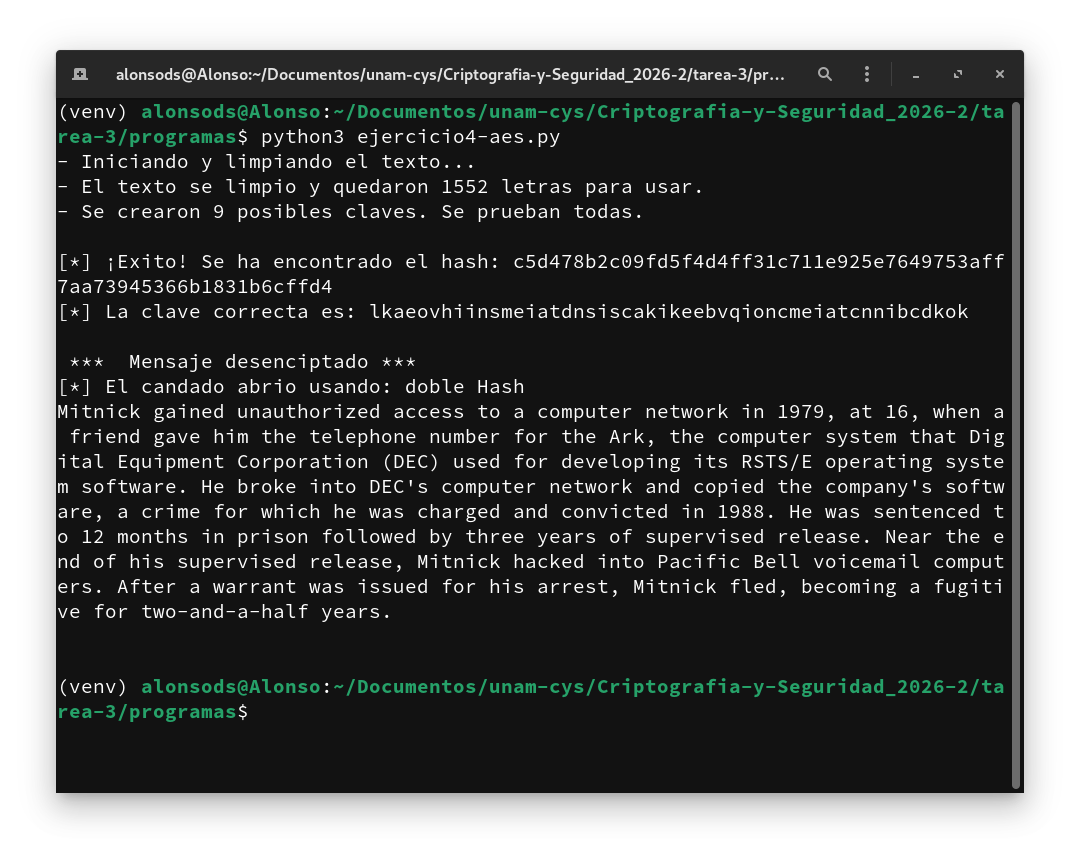
\includegraphics[scale=0.4]{imagenes/Capturas/ej-4.png}
	\label{fig:Ejecucion-ej-4}
	\caption{Ejecución del programa \textbf{ejercicio4-aes.py}}
\end{figure}

\newpage
\section*{Problema 5: El gran secreto dentro de una imagen}
El objetivo de este problema fue aplicar los principios esteganográficos mediante los comandados dados sobre el archivo de imagen \texttt{mao-shi.jpg} y descubrir una bandera (flag) secreta.
Para la resolución de este problema, se utilizó la máquina virtual de Kali Linux y se siguieron los siguientes pasos:
\begin{enumerate}
	\item Inicialmente, fue necesario instalar el software requerido: \texttt{steghide} y \texttt{jp2a}. Steghide es una herramienta clásica de línea de comandos que utiliza un algoritmo esteganográfico para incrustar o extraer datos de archivos multimedia (como JPEG o BMP), protegiéndolos adicionalmente con una contraseña. Por otro lado, jp2a es un conversor que permite transformar imágenes a arte ASCII.
	\begin{lstlisting}[language=bash, numbers=none]
		$ sudo apt-get update
		$ sudo apt-get install steghide jp2a\end{lstlisting}
	\begin{figure}[H]
		\centering
		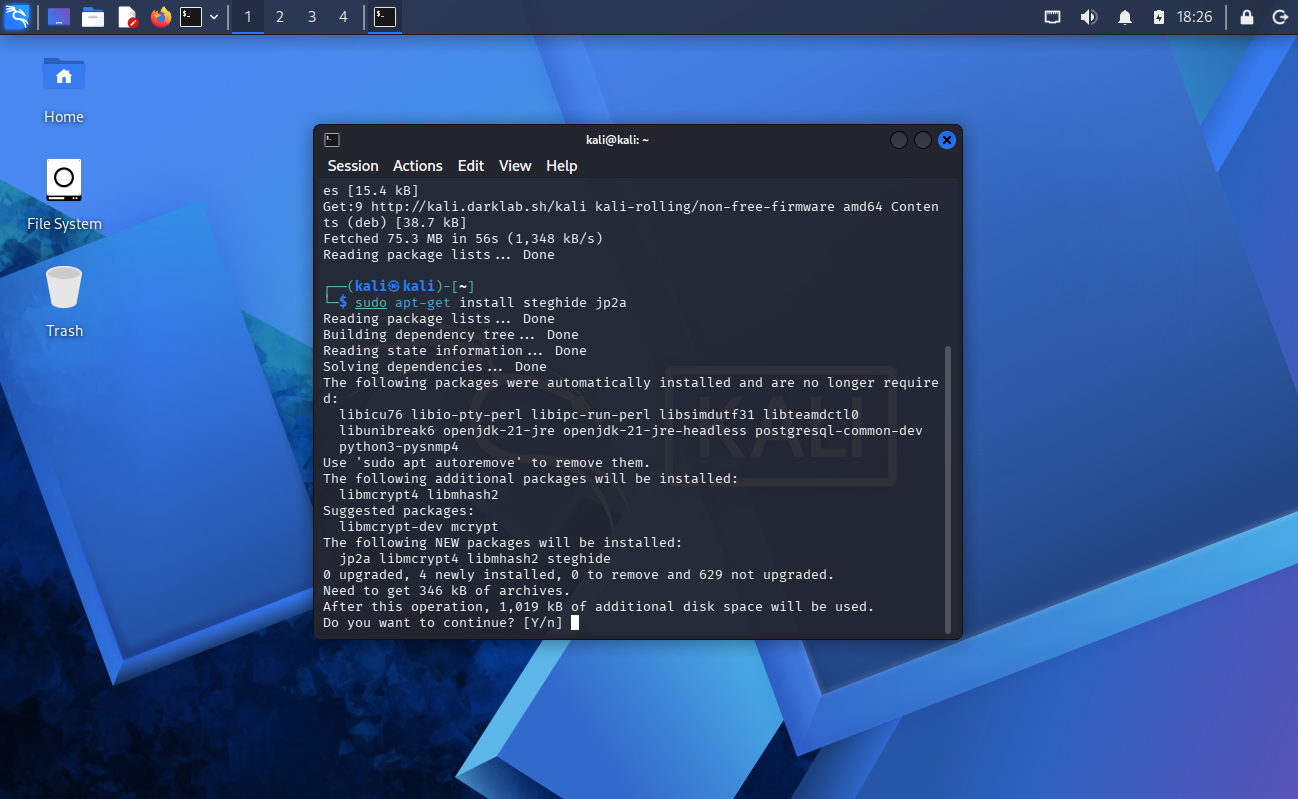
\includegraphics[scale=0.35]{imagenes/Capturas/ej-5-1.png}
		\label{fig:Ejecucion-ej-5-1}
		\caption{Instalación de \texttt{steghide} y \texttt{jp2a}.}
	\end{figure}
	
	\item Una vez instaladas las herramientas, se procedió a inspeccionar la imagen objetivo. Sabiendo que la imagen contenía datos inyectados, se ejecutó el comando de extracción de steghide sobre el archivo \texttt{mao-shi.jpg}. Al solicitar la frase de contraseña, se introdujo la credencial proporcionada: \textbf{eje4}.
	El algoritmo descifró y extrajo exitosamente un archivo oculto, generando en nuestro directorio local un ejecutable de bash llamado \texttt{silent.sh}.
	\begin{lstlisting}[language=bash, numbers=none]
		$ steghide extract -sf mao-shi.jpg	\end{lstlisting}
	\begin{figure}[H]
		\centering
		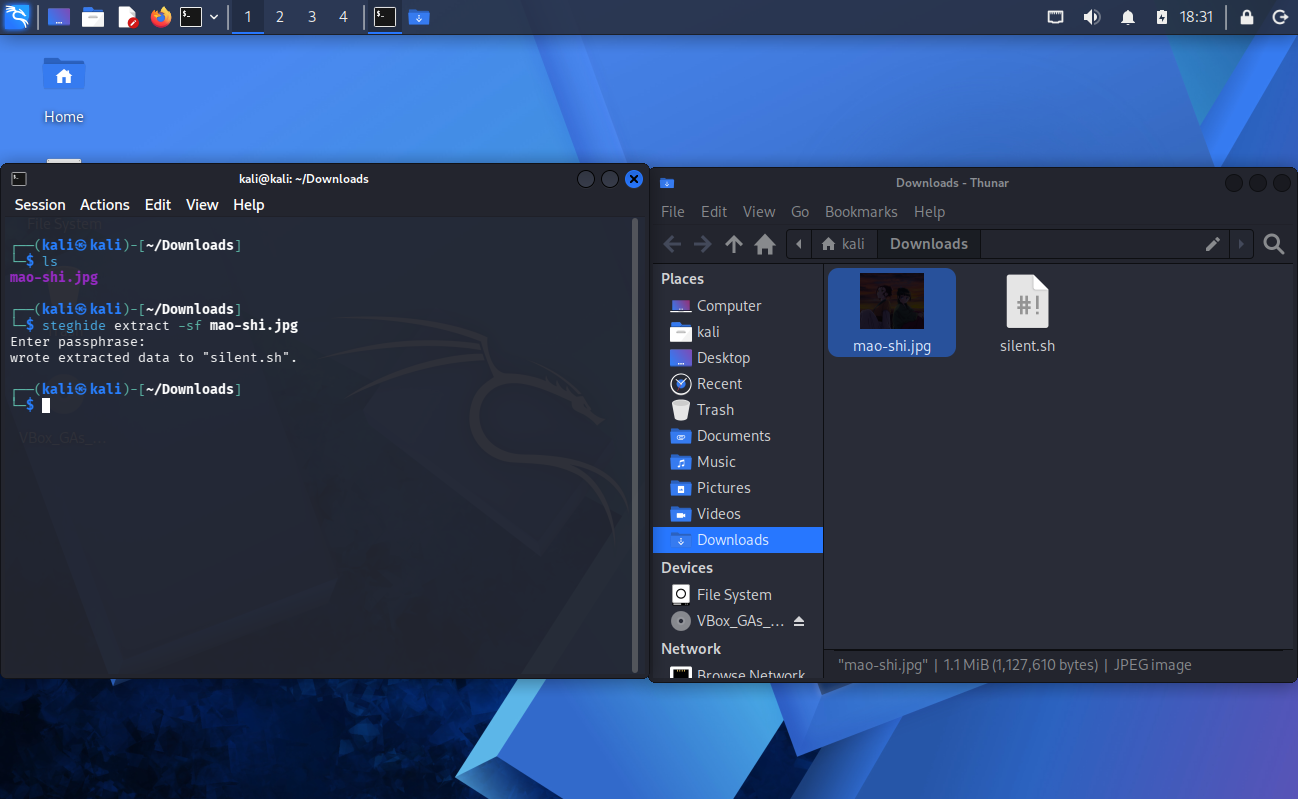
\includegraphics[scale=0.35]{imagenes/Capturas/ej-5-2.png}
		\label{fig:Ejecucion-ej-5-2}
		\caption{Extracción de datos ocultos}
	\end{figure}
	
	\item Tras otorgarle permisos de ejecución al archivo \texttt{silent.sh}, se procedió a ejecutarlo en la terminal. El resultado de este script fue la generación de un archivo \texttt{index.html}.
	\begin{lstlisting}[language=bash, numbers=none]
		$ chmod +x silent.sh
		$ ./silent.sh	\end{lstlisting}
	\begin{figure}[H]
		\centering
		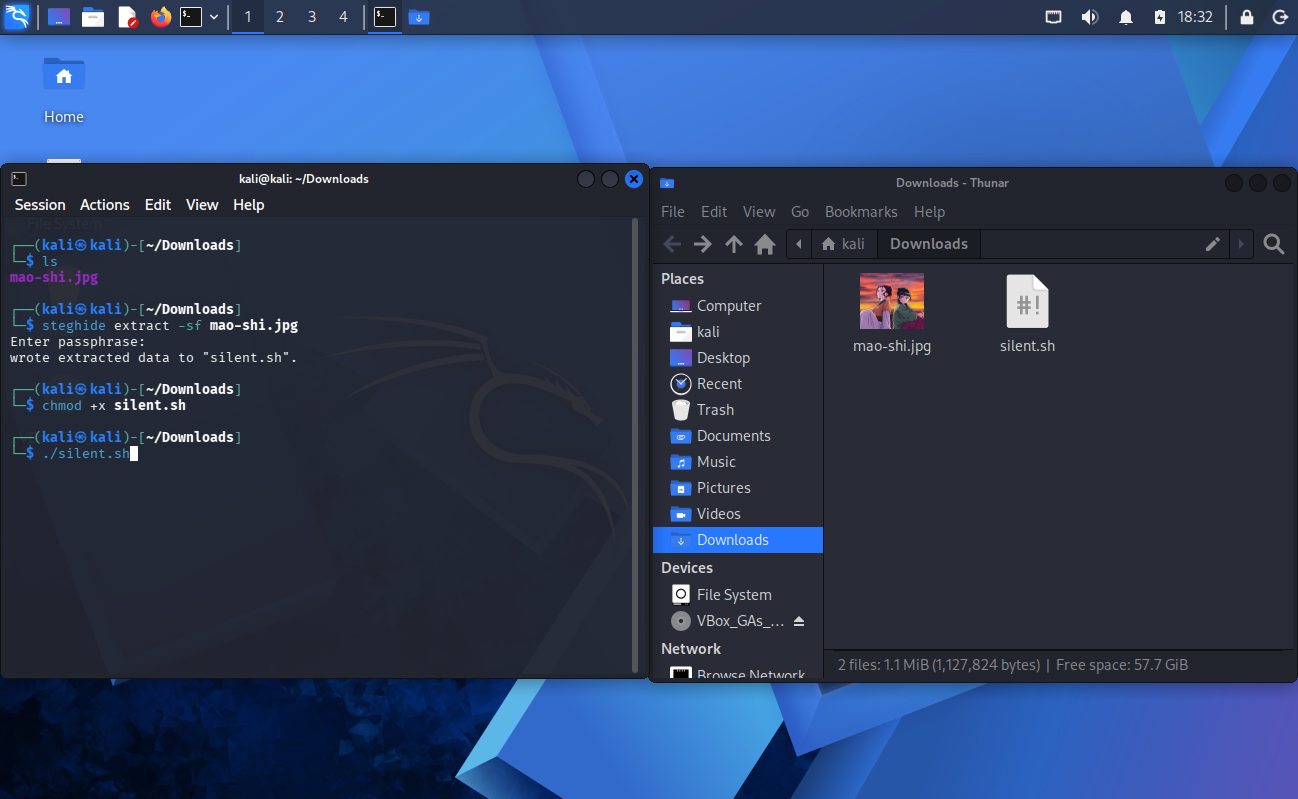
\includegraphics[scale=0.35]{imagenes/Capturas/ej-5-3.png}
		\label{fig:Ejecucion-ej-5-3}
		\caption{Permisos y ejecución de \texttt{silent.sh}.}
	\end{figure}
	
	\item Al abrir el archivo \texttt{index.html} en el navegador, la pantalla principal mostraba el diseño en arte ASCII sobre un fondo negro. Sin embargo, tanto al seguir jugando con la selección de texto en el navegador, o bien, al realizar una inspección directa del código fuente del HTML, se descubrió al final del documento, el siguiente texto:
	\begin{lstlisting}[language=bash, numbers=none]
		FLAG{s73g4n0gr4phy_15_h1dd3n}	\end{lstlisting}
	\begin{figure}[H]
		\centering
		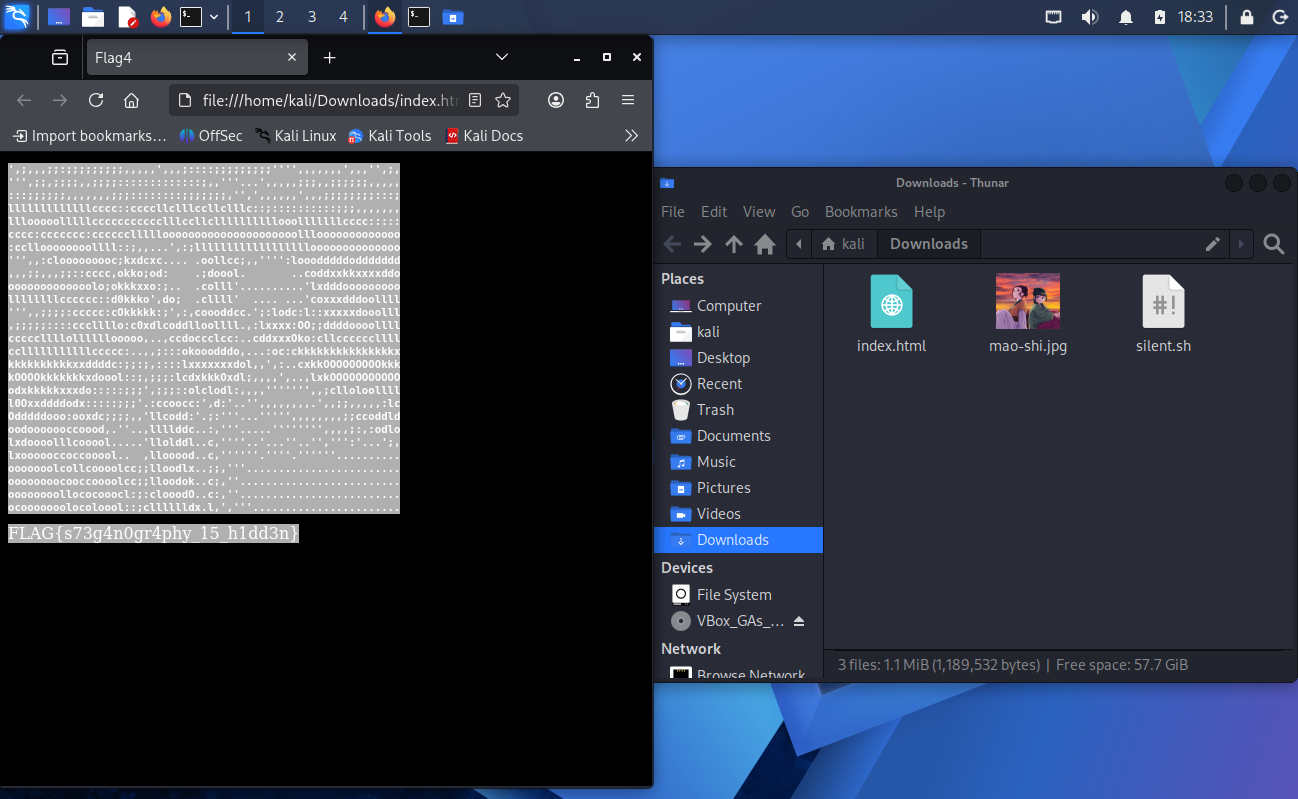
\includegraphics[scale=0.35]{imagenes/Capturas/ej-5-5.png}
		\label{fig:Ejecucion-ej-5-5}
		\caption{Inspección y descubrimiento de la bandera.}
	\end{figure}
	
\end{enumerate}
Este ejercicio demostró cómo simples archivos multimedia pueden utilizarse para cargar información o introducir scripts (.sh) en sistemas objetivo sin levantar sospechas de firewalls o antivirus, ya que a nivel de red y de sistema de archivos, el archivo original es indistinguible de una imagen JPEG normal. 

La bandera recuperada fue: \textbf{\texttt{FLAG{s73g4n0gr4phy\_15\_h1dd3n}}}


\section*{Problema 6: Una gran tormenta se avecina}
El objetivo de este problema es comprender la naturaleza y el impacto de los ataques de Denegación de Servicio (DoS) y su variante distribuida (DDoS). Específicamente, se simuló un ataque de Inundación SYN (SYN Flood) contra un servidor web. Este tipo de ataque explota el diseño Three-way Handshake del protocolo TCP, enviando una cantidad masiva de solicitudes de conexión (SYN) sin llegar a completarlas nunca (ACK), con el fin de agotar la memoria y los recursos del servidor víctima hasta dejarlo inoperante.

Para la realización de esta ejercicio, se adaptó el entorno utilizando una máquina virtual con Fedora 43 configurada en modo adaptador puente (Bridged) actuando como servidor víctima (con los servicios \texttt{httpd}, \texttt{vsftpd} y \texttt{sshd} activos), y una maquina física con Fedora 42 que actúa como atacante con la herramienta hping3 instalada.
\begin{figure}[H]
	\centering
	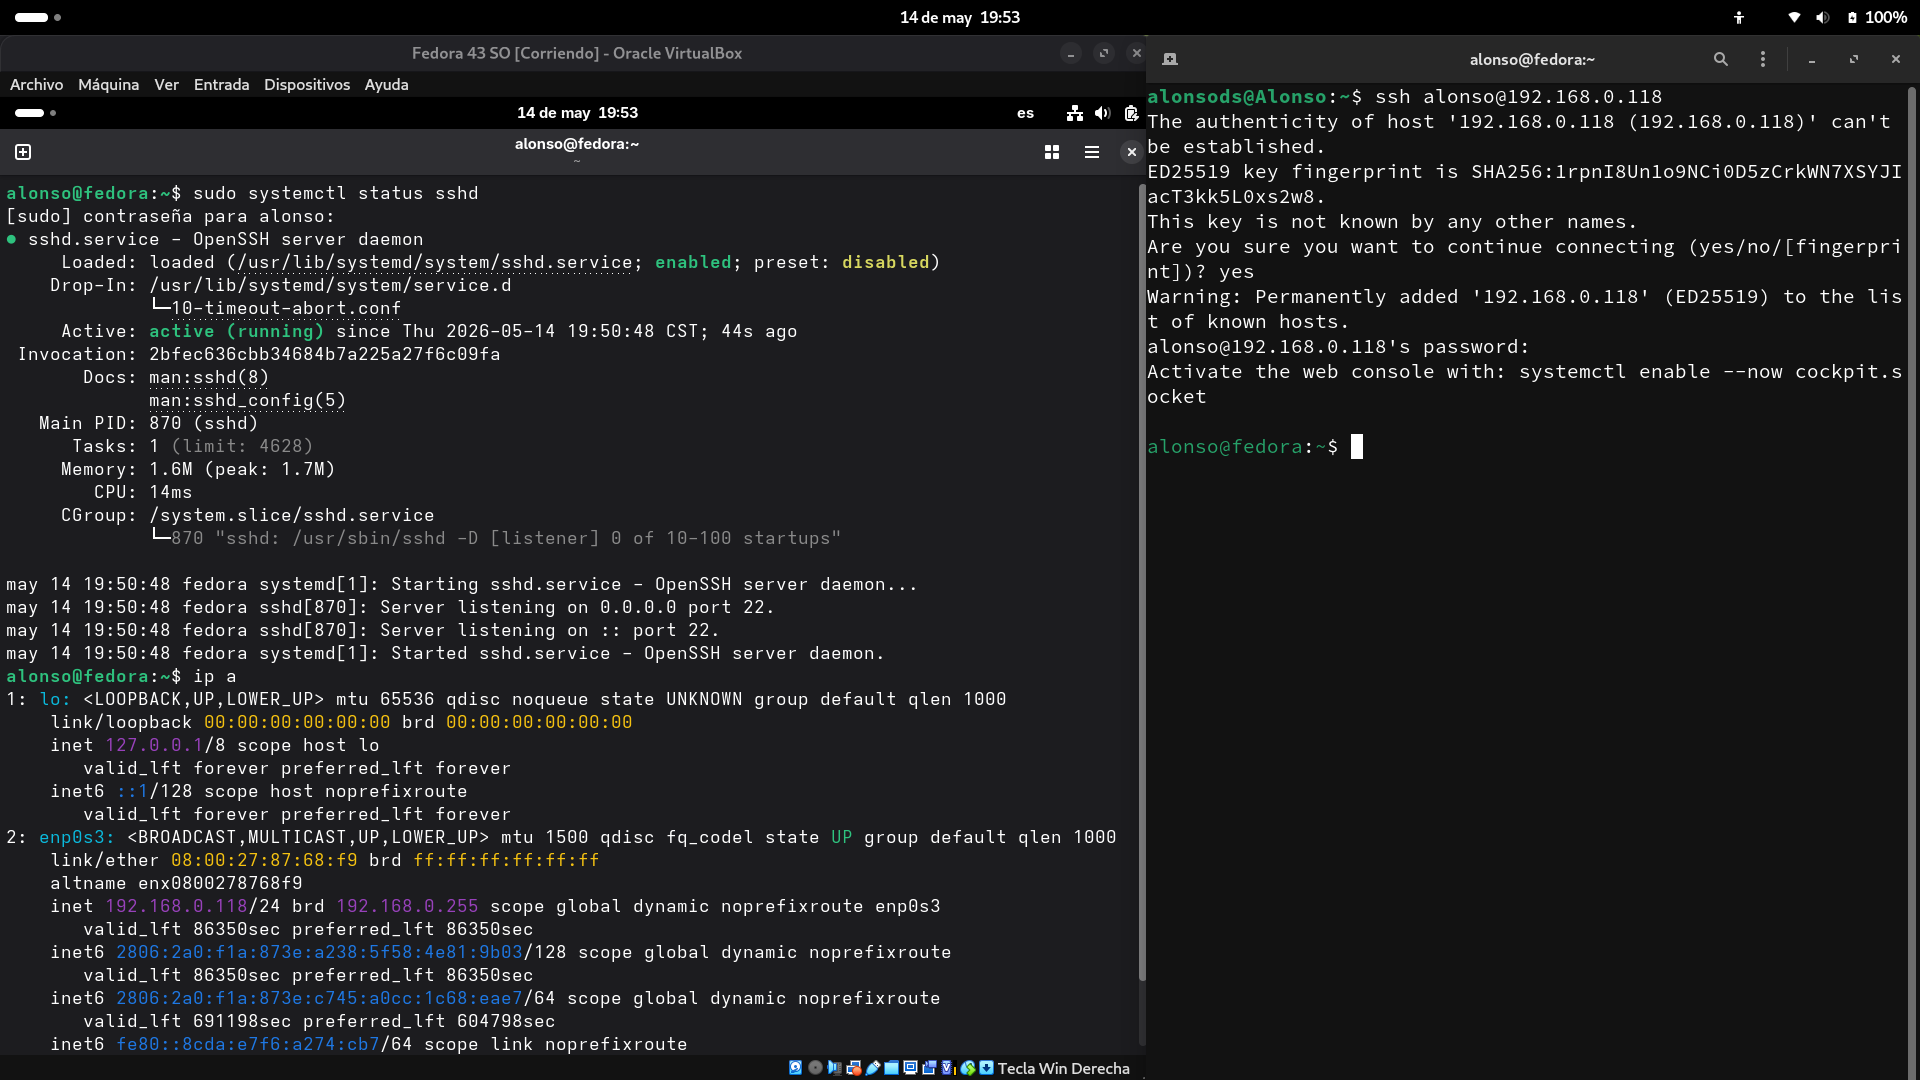
\includegraphics[scale=0.25]{imagenes/Capturas/ej-6-1.png}
	\label{fig:Ejecucion-ej-6-1}
	\caption{Prueba de conexión SSH entre la máquina virtual (victima) y máquina física (atacante) }
\end{figure}
Con el comando \texttt{ip a}, obtenemos la IP de nuestra máquina virtual: \textbf{192.168.0.118}.\\
Instalamos todas las bibliotecas necesarias en nuestra máquina víctima y activamos los servicios. El repositorio brinda los comandos para Debian, por lo que los comandos en Fedora son:
\begin{lstlisting}[language=bash, numbers=none]
	# Instalacion de servicios en Fedora (reemplaza a apt-get)
	sudo dnf update
	sudo dnf install httpd vsftpd openssh-server wireshark
	
	# Iniciar los servicios (Apache se llama httpd en Fedora)
	sudo systemctl start httpd
	sudo systemctl start vsftpd
	sudo systemctl start sshd
\end{lstlisting}
\begin{figure}[H]
	\centering
	\vspace{-30pt}
	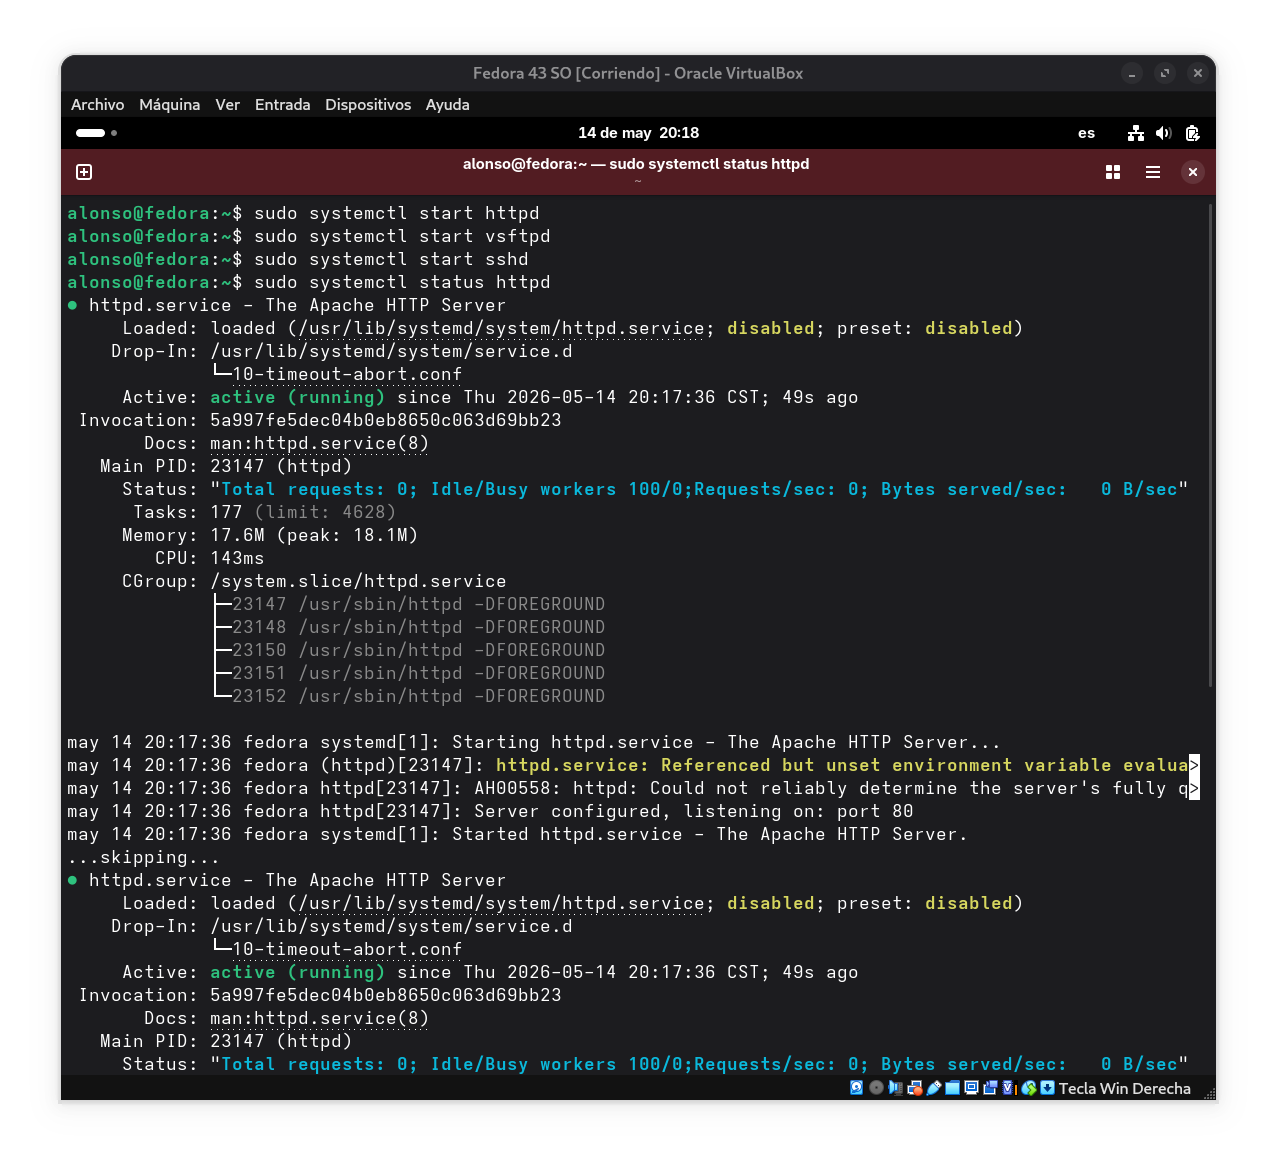
\includegraphics[scale=0.3]{imagenes/Capturas/ej-6-2.png}
	\label{fig:Ejecucion-ej-6-2}
	\vspace{-20pt}
	\caption{Verificación de estatus de los servicios (en VM)}
\end{figure}
\begin{figure}[H]
	\centering
	\vspace{-30pt}
	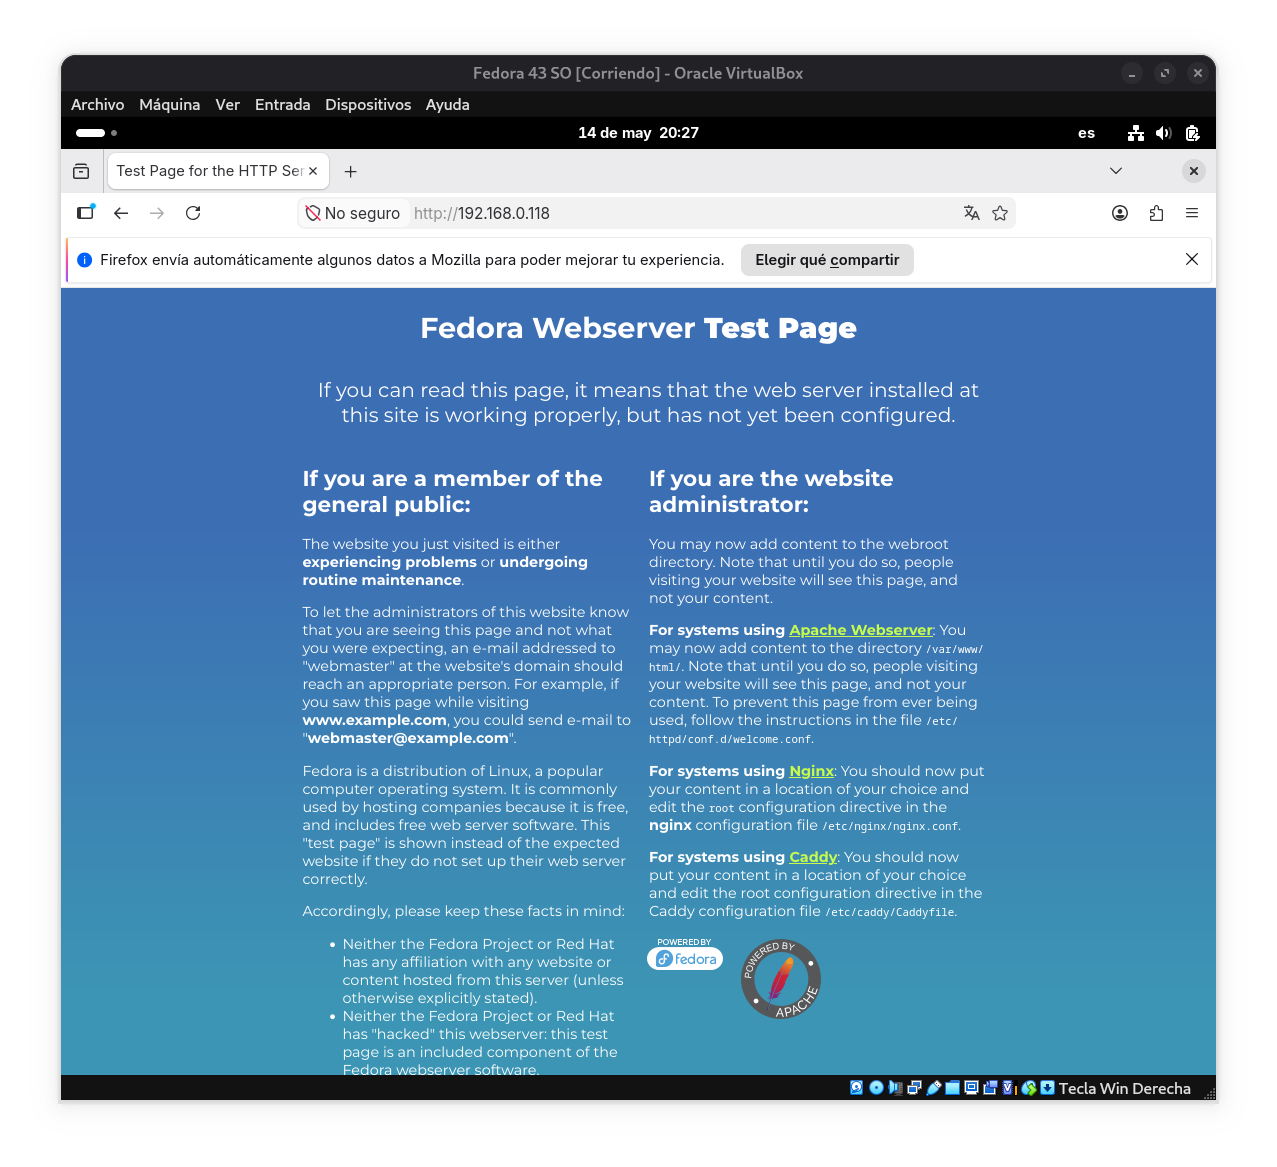
\includegraphics[scale=0.3]{imagenes/Capturas/ej-6-3.png}
	\label{fig:Ejecucion-ej-6-3}
	\vspace{-20pt}
	\caption{Comprobación del servicio Apache activo desde el navegador (en VM)}
	\vspace{-20pt}
\end{figure}

Antes de ejecutar el ataque, fue necesario confirmar que el objetivo tenía los puertos correctos abiertos. Desde la máquina atacante se ejecutó un escaneo de los primeros 1024 puertos utilizando \texttt{hping3}:
\begin{lstlisting}[language=bash, numbers=none]
	sudo hping3 --scan 1-1024 -S 192.168.0.118
\end{lstlisting}
Este comando envía un paquete TCP con la bandera SYN a los primeros 1024 puertos. Si el puerto está abierto, la máquina víctima responde con un SYN-ACK.
\begin{figure}[H]
	\centering
	\vspace{-10pt}
	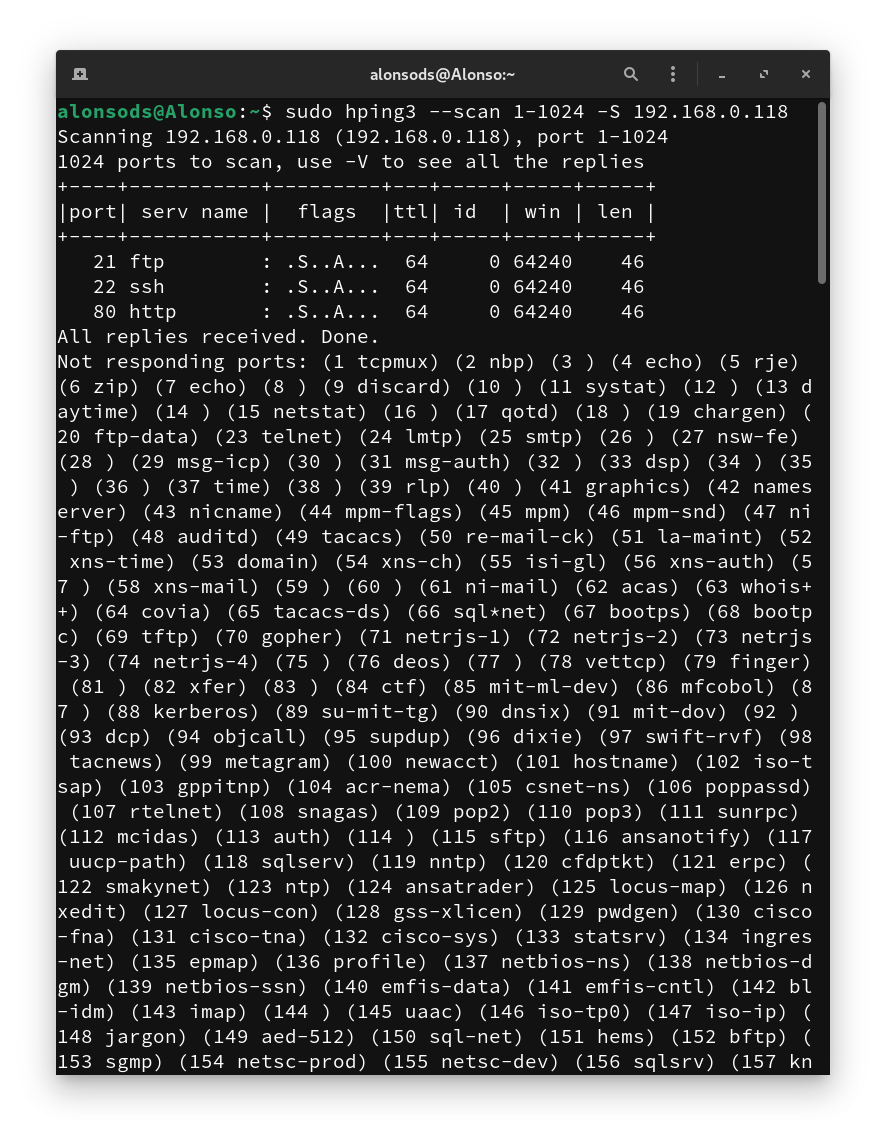
\includegraphics[scale=0.35]{imagenes/Capturas/ej-6-4.png}
	\label{fig:Ejecucion-ej-6-4}
	\vspace{-20pt}
	\caption{Escaneo de puertos abiertos con \texttt{hping3}}
\end{figure}
Como observación adicional, estos mismos puertos abiertos también pueden ser escaneados con \texttt{nmap}.
\begin{lstlisting}[language=bash, numbers=none]
	nmap -p 1-1024 192.168.0.118
\end{lstlisting}
\begin{figure}[H]
	\centering
	\vspace{-20pt}
	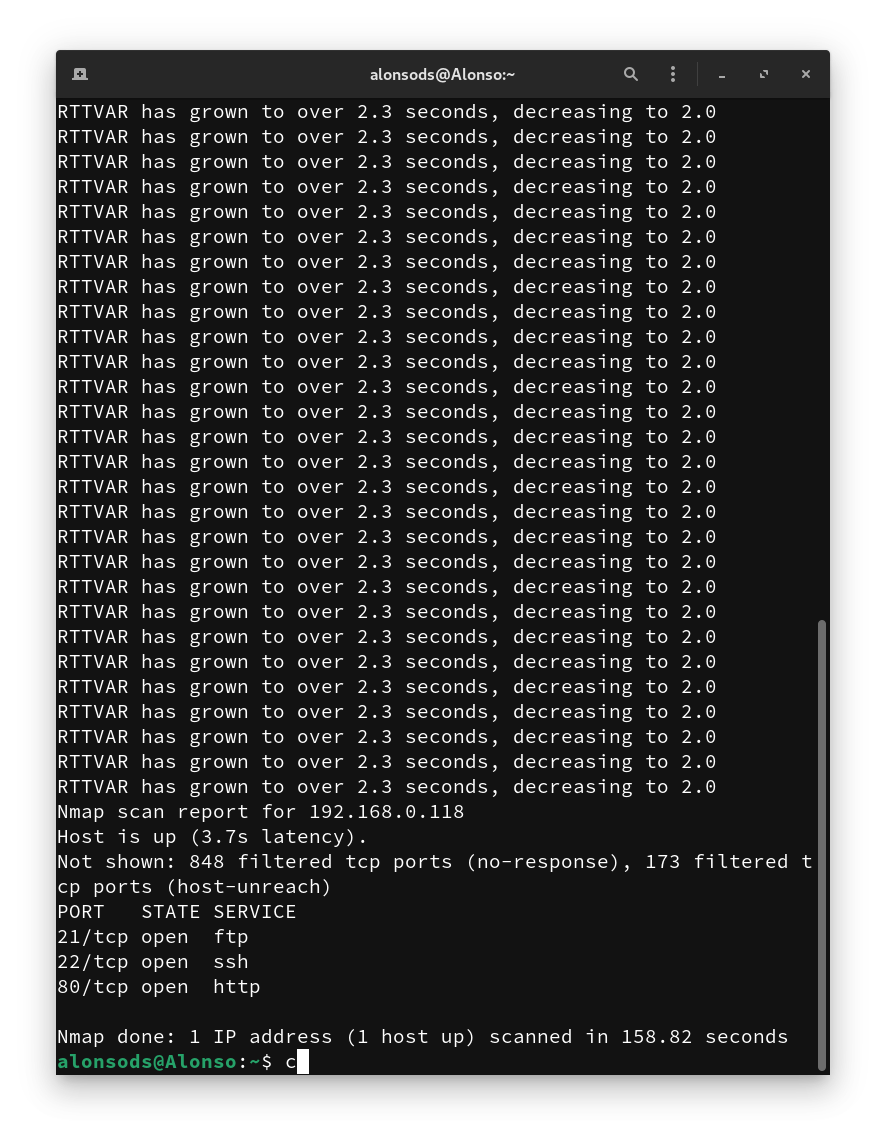
\includegraphics[scale=0.35]{imagenes/Capturas/ej-6-5.png}
	\label{fig:Ejecucion-ej-6-5}
	\vspace{-20pt}
	\caption{Escaneo de puertos abiertos con \texttt{nmap}}
\end{figure}
Ejecutamos Wireshark en nuestra máquiva virtual y luego seleccionamos la interfaz de red que se esta usando.
\begin{figure}[H]
	\centering
	\vspace{-30pt}
	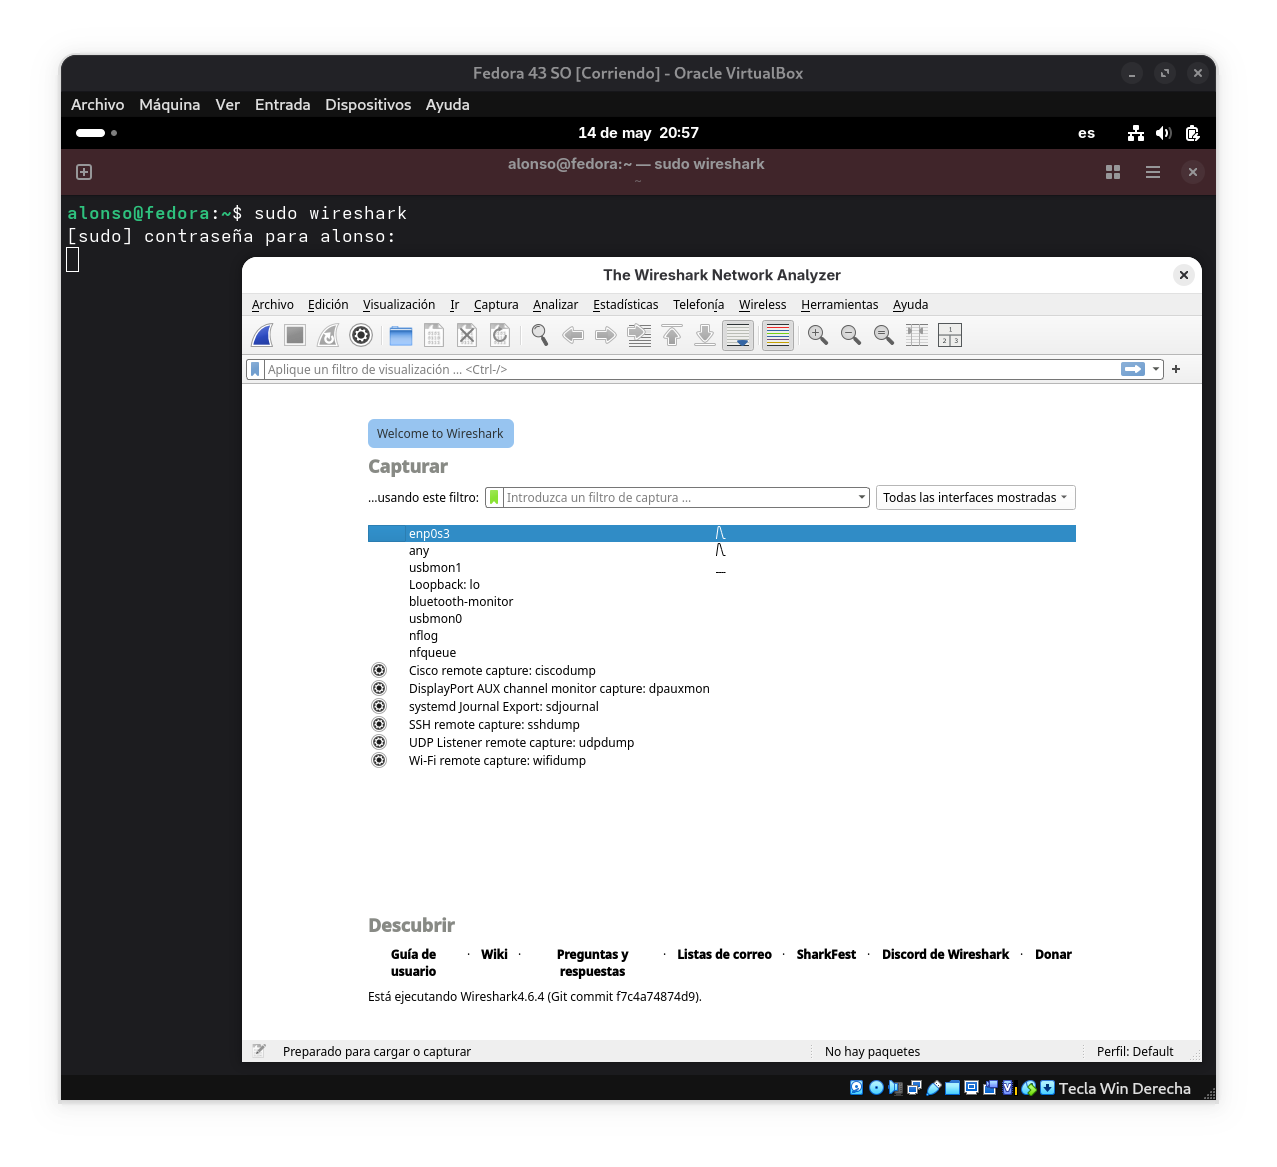
\includegraphics[scale=0.3]{imagenes/Capturas/ej-6-6.png}
	\label{fig:Ejecucion-ej-6-6}
	\vspace{-20pt}
	\caption{Ejecución de Wireshark (en VM)}
\end{figure}
\begin{figure}[H]
	\centering
	\vspace{-30pt}
	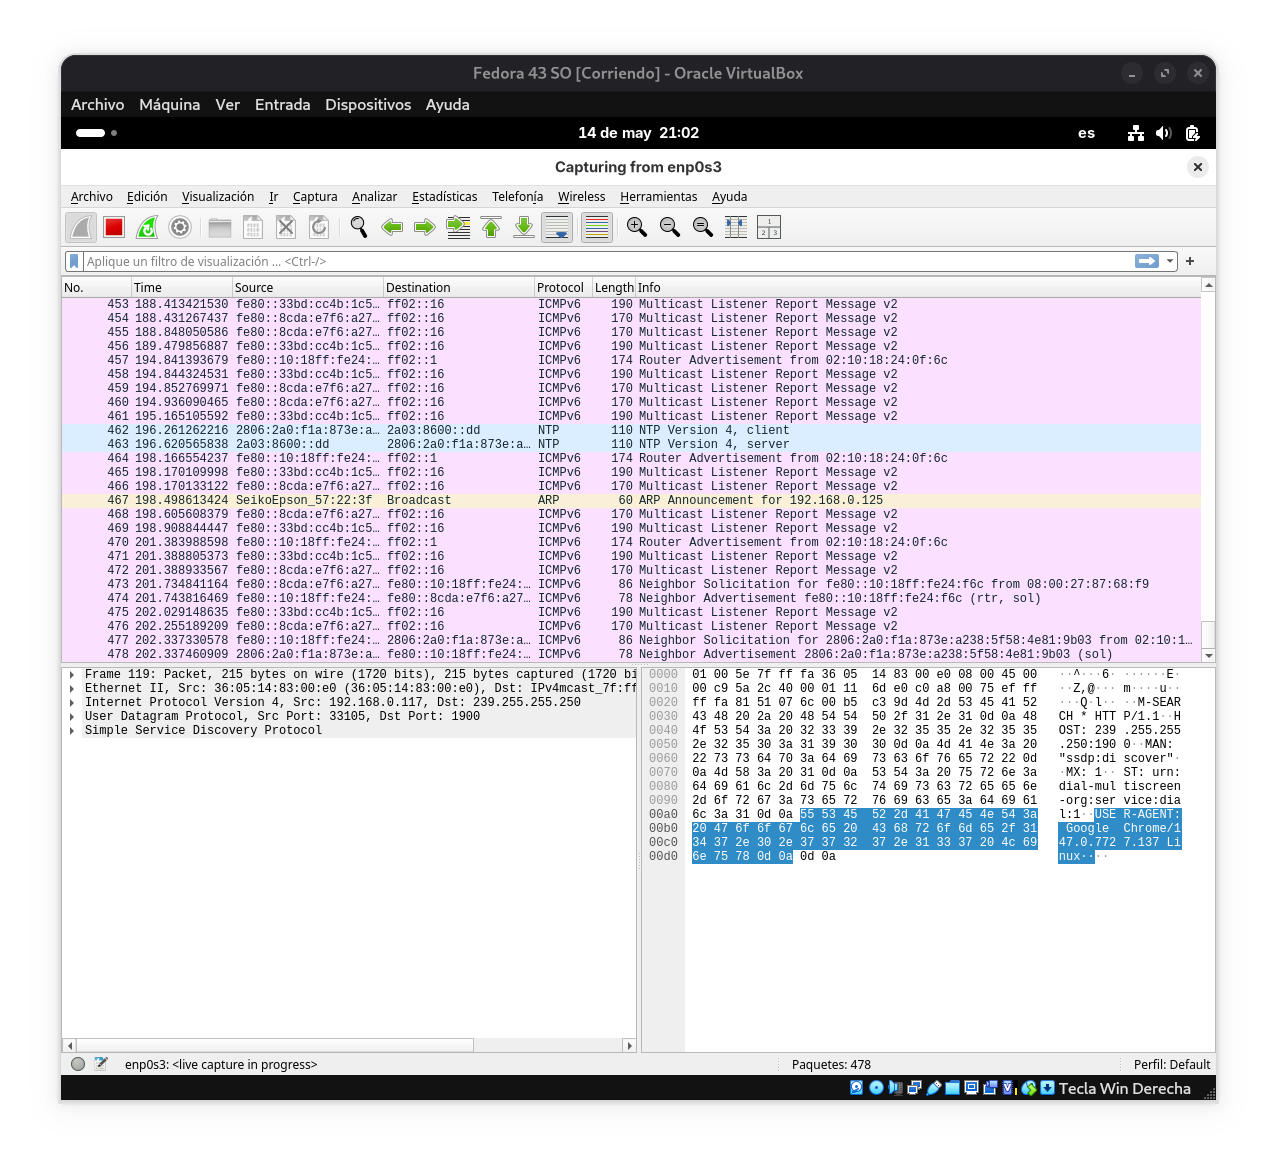
\includegraphics[scale=0.3]{imagenes/Capturas/ej-6-7.png}
	\label{fig:Ejecucion-ej-6-7}
	\vspace{-20pt}
	\caption{Se elige la interfaz de red para visualizar el tráfico de paquetes}
	\vspace{-20pt}
\end{figure}
Una vez identificado el puerto 80 abierto, se procedió a lanzar el primer ataque de inundación (flood) y se monitoreó el tráfico en la máquina víctima utilizando Wireshark.
\begin{lstlisting}[language=bash, numbers=none]
	sudo hping3 -S -V --flood -p 80 192.168.0.118
\end{lstlisting}
Observamos que la red se satura instantáneamente con una gran cantidad de paquetes que ingresan a rápida velocidad, en partícular, este tráfico TCP va dirigido exclusivamente al puerto 80 con la bandera [SYN] activada. Todos los paquetes maliciosos provienen de la misma dirección IP (la de nuestra máquina atacante). \\
Podemos notar que a diferencia del tráfico legítimo, en donde existe el saludo completo: SYN (cliente) $\rightarrow$ SYN-ACK (servidor) $\rightarrow$ ACK (cliente), seguido de la transferencia de datos; en este tráfico malicioso, el servidor responde rápidamente con [SYN, ACK], pero el atacante ignora estas respuestas y jamás envía el paquete ACK final, dejando las conexiones abiertas.
\begin{figure}[H]
	\centering
	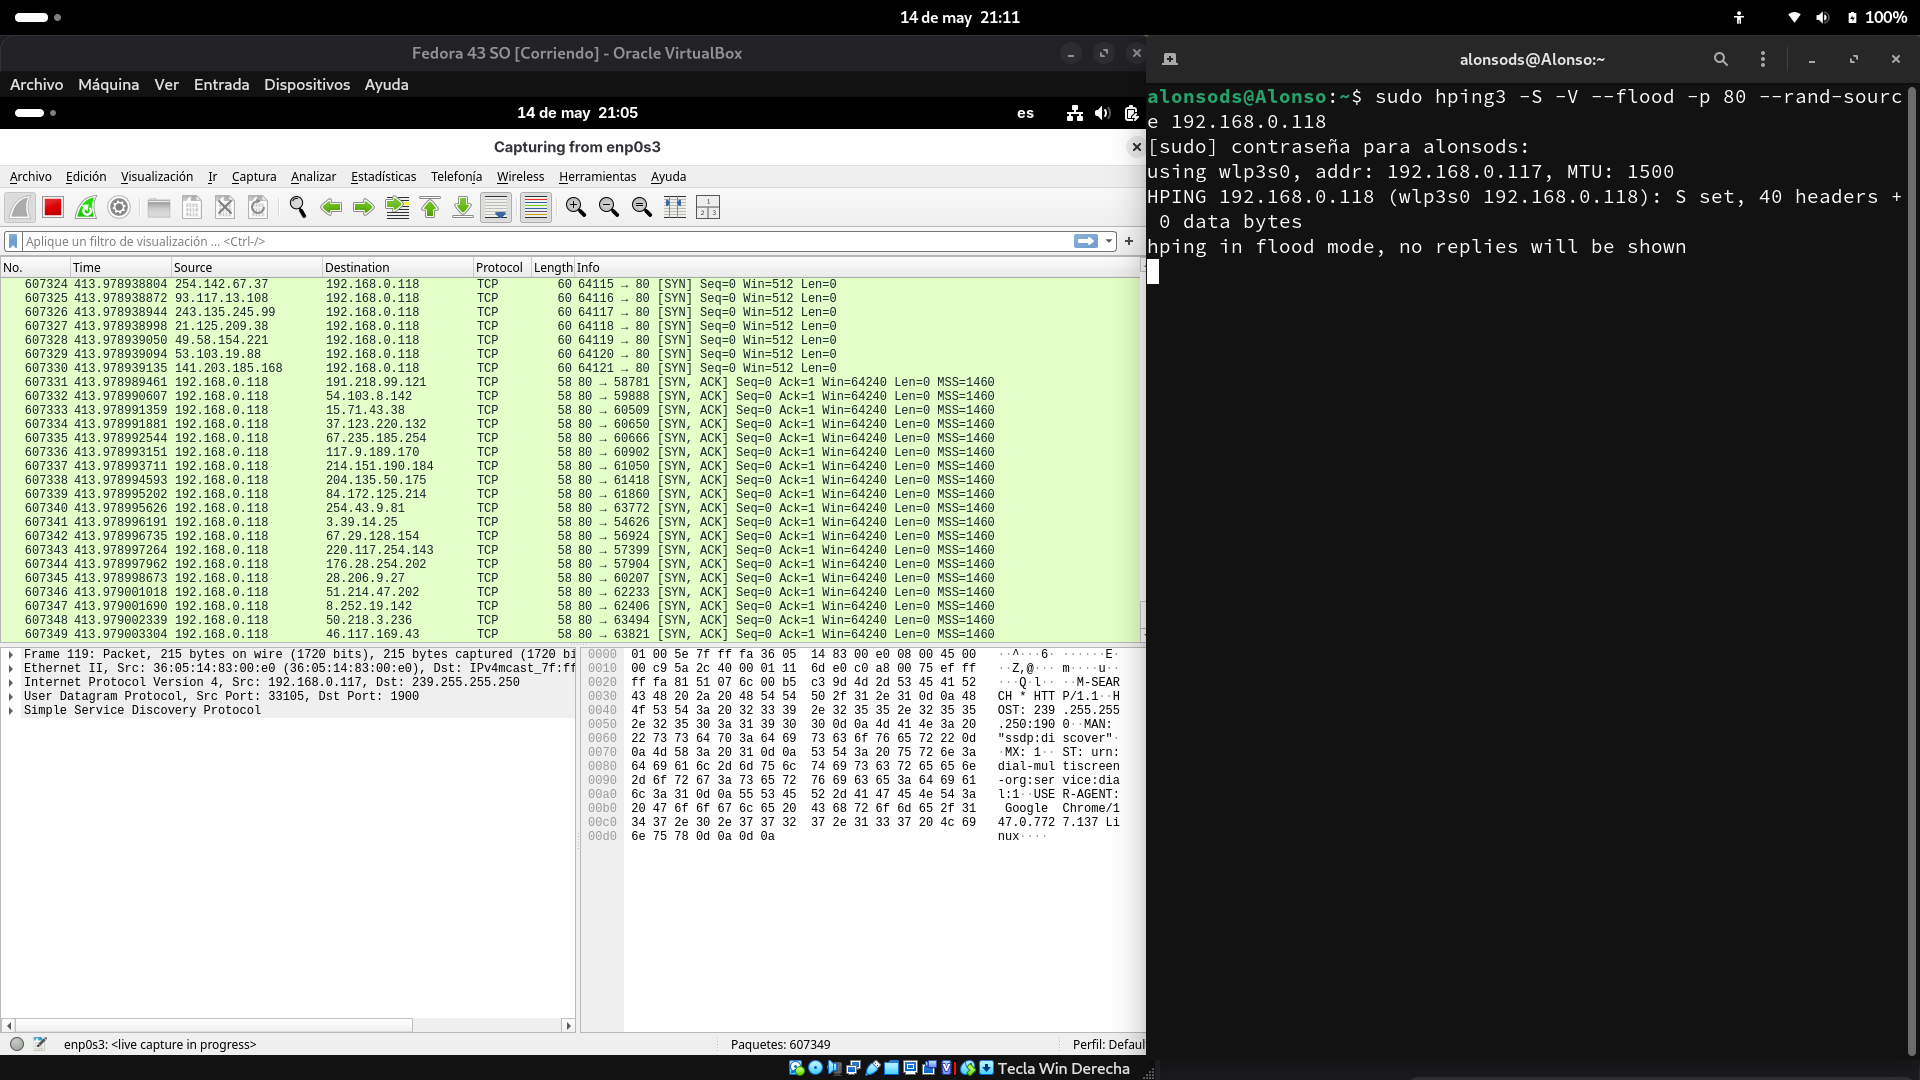
\includegraphics[scale=0.25]{imagenes/Capturas/ej-6-8.png}
	\label{fig:Ejecucion-ej-6-8}
	\caption{Ataque DDoS visto desde Wireshark}
\end{figure}
\begin{figure}[H]
	\centering
	\vspace{-40pt}
	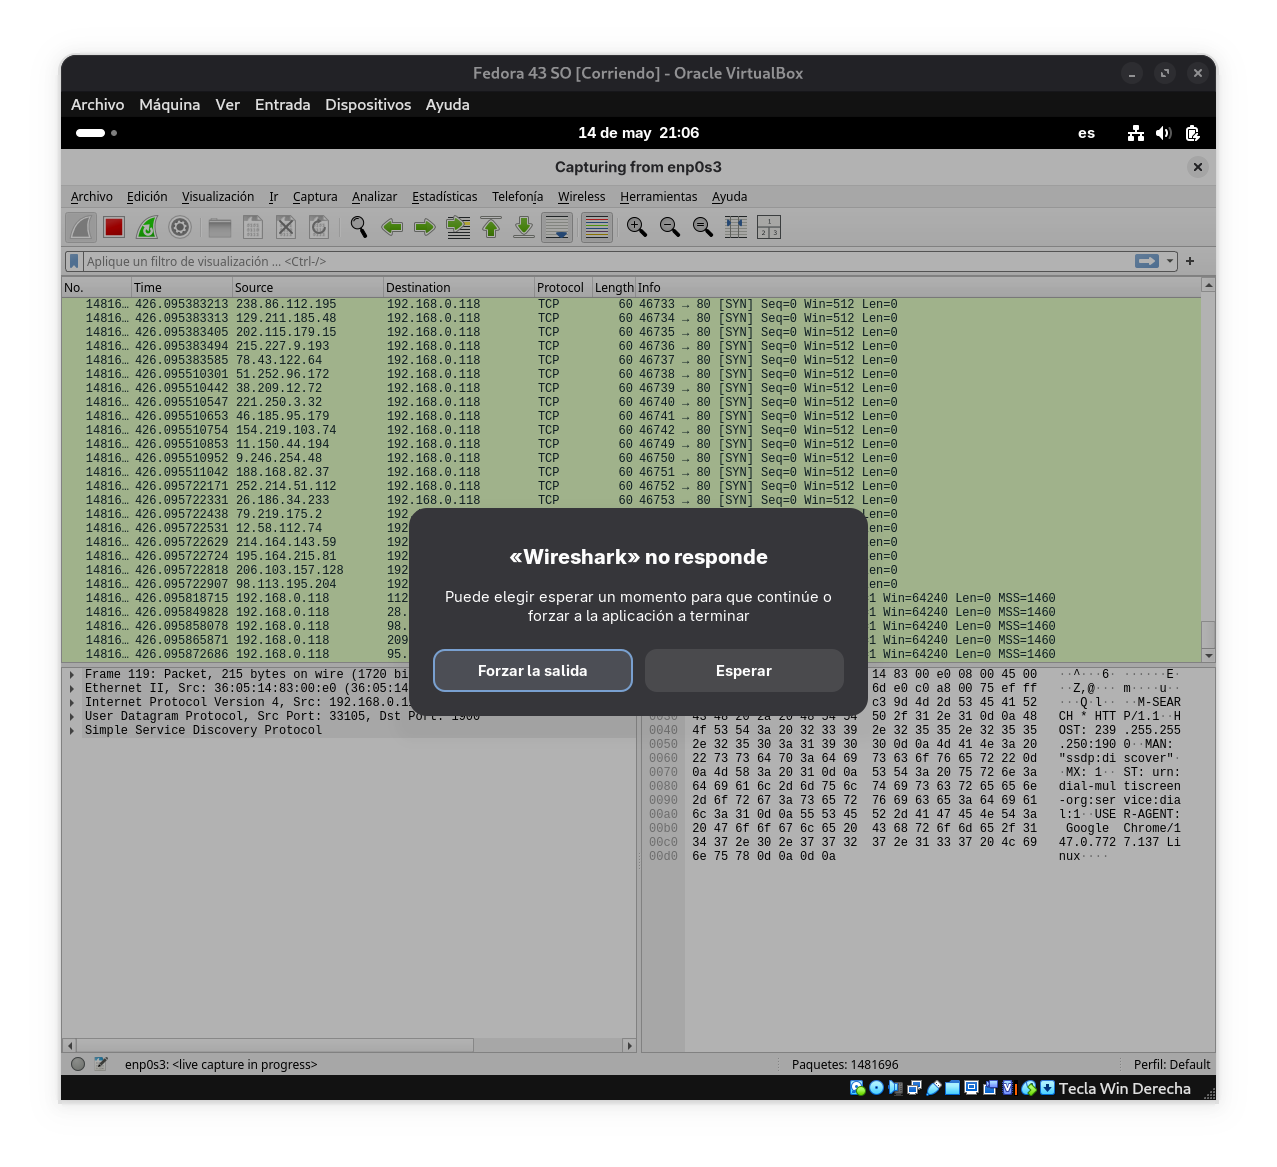
\includegraphics[scale=0.30]{imagenes/Capturas/ej-6-9.png}
	\label{fig:Ejecucion-ej-6-9}
	\vspace{-20pt}
	\caption{Crasheo en Wiresehark a causa de la cantidad de tráfico de red entrante}
\end{figure}
\begin{figure}[H]
	\centering
	\vspace{-20pt}
	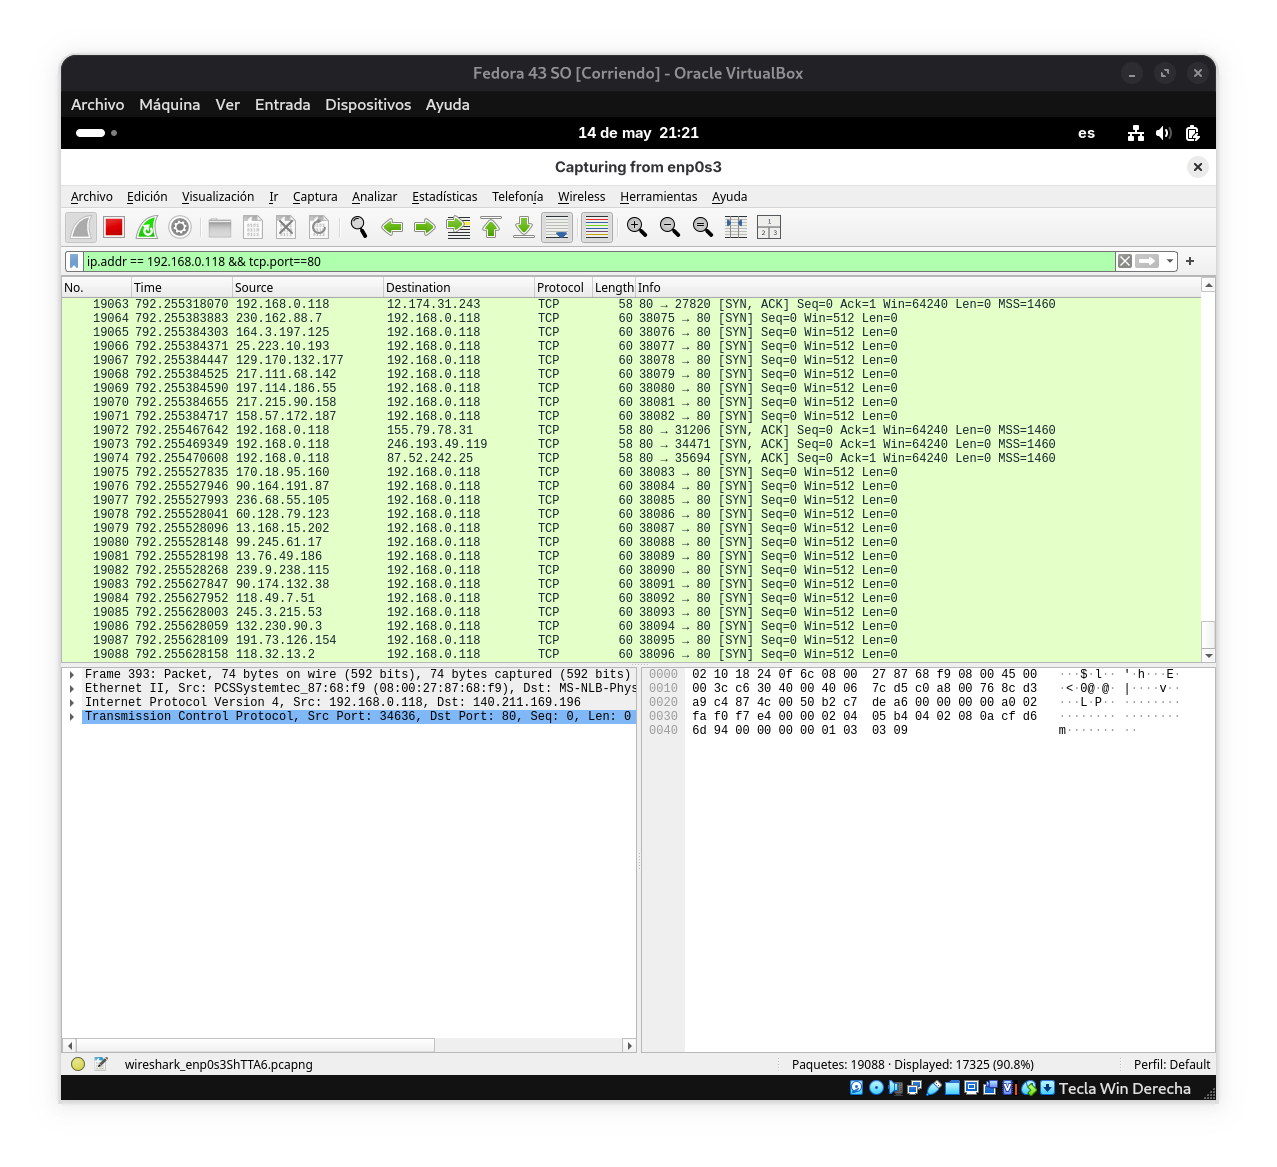
\includegraphics[scale=0.30]{imagenes/Capturas/ej-6-10.png}
	\label{fig:Ejecucion-ej-6-10}
	\vspace{-20pt}
	\caption{Nuevo ataque pero con filtro \texttt{ip.addr == 192.168.0.118 \&\& tcp.port == 80} }
	\vspace{-20pt}
\end{figure}

Al aplicar el filtro de visualización en Wireshark, aislamos el tráfico dirigido al servidor web. Observamos nuevamente una alta cantidad de paquetes [SYN], pero con una diferencia en la columna de origen (Source). A diferencia del primer ataque donde la IP atacante era visible y constante, ahora cada paquete entrante proviene de una dirección IP completamente distinta.

Este ejercicio demostró la vulnerabilidad inherente de los protocolos de conexión cuando se enfrentan a volúmenes de tráfico diseñados para agotar sus recursos.

\section*{Problema 7: ¡Hey! No mires más de lo necesario.}
Para este ejercicio se pudo visualizar la importancia del cifrado en las conexiones remotas, contrastando un protocolo antiguo e inseguro como Telnet, contra el estándar actual que es Secure Shell (SSH). Telnet permite el acceso en modo terminal a una máquina remota, sin embargo, carece de mecanismos de confidencialidad. Por su parte, SSH (Secure Shell) establece un canal seguro donde toda la información transmitida se encuentra cifrada. Mediante la interceptación de paquetes con Wireshark, se pondrá en práctica por qué el uso de protocolos con texto plano representa una vulnerabilidad crítica.

En esta ocasión, el servidor víctima opera en la VM Fedora 42 (en lugar de Debian) con ip \textbf{192.168.0.118}. Mientras que nuestra máquina atacante será en la VM de Kali Linux.
\begin{figure}[H]
	\centering
	\vspace{0pt}
	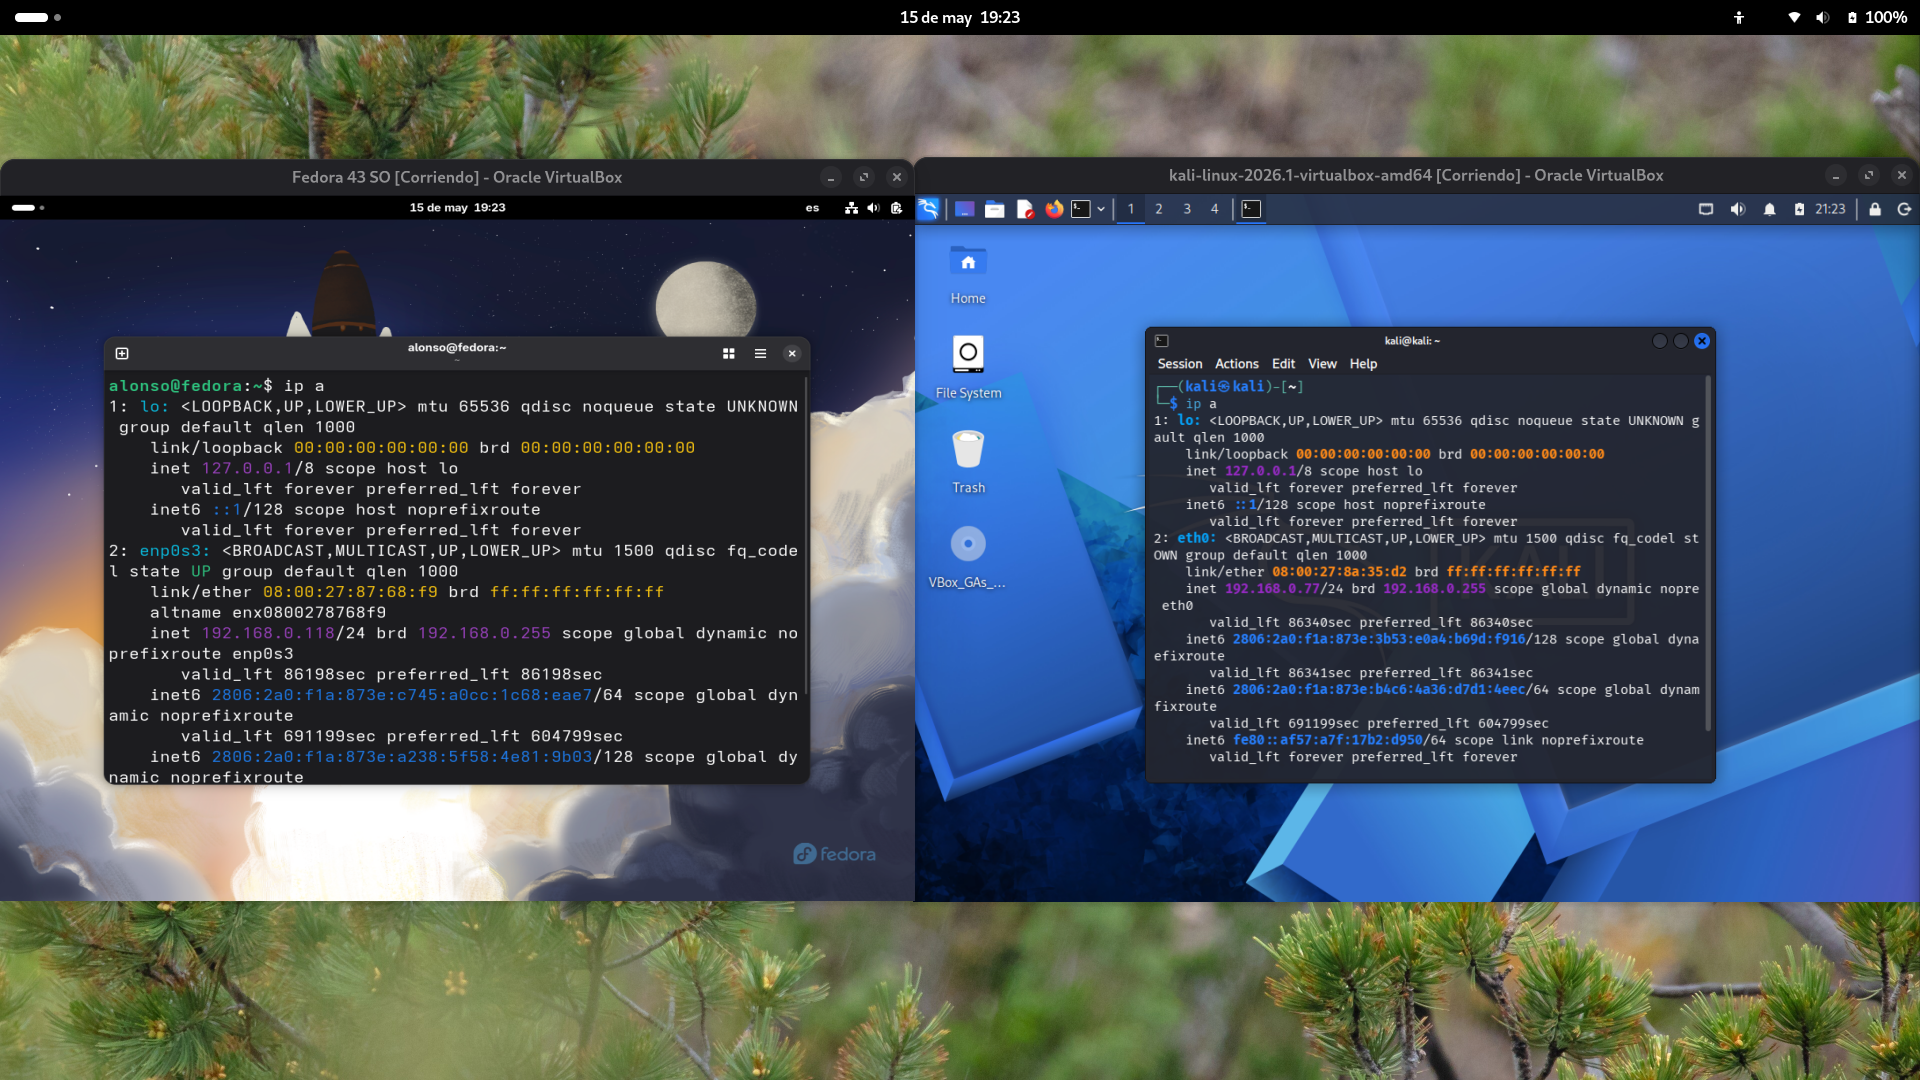
\includegraphics[scale=0.25]{imagenes/Capturas/ej-7-1.png}
	\label{fig:Ejecucion-ej-7-1}
	\vspace{-20pt}
	\caption{Máquina victima (Fedora) y máquina atacante (Kali Linux)}
	\vspace{-20pt}
\end{figure}

Debido a que el servidor víctima funciona con Fedora 42, una distribución Linux moderna, el gestor de demonios de red heredado (\texttt{xinetd}) utilizado en las instrucciones originales ha sido descontinuado y eliminado de sus repositorios oficiales. Por lo tanto con ayuda Gemini, se adaptaron los comandos para Fedora para la iniicialización y configuración del entorno:
\subsubsection*{Instalación de paquetes}
\begin{lstlisting}[language=bash, numbers=none]
	sudo dnf update
	sudo dnf install telnet-server telnet openssh-server
\end{lstlisting}
\subsubsection*{Inicialización de servicios}
\begin{lstlisting}[language=bash, numbers=none]
	sudo systemctl daemon-reload
	sudo systemctl enable telnet.socket
	sudo systemctl restart telnet.socket
	sudo systemctl enable sshd
\end{lstlisting}
\subsubsection*{Configuración de Firewall nativo}
\begin{lstlisting}[language=bash, numbers=none]
	sudo firewall-cmd --add-service=telnet
	sudo firewall-cmd --add-service=ssh
\end{lstlisting}
Preparamos Wireshark en Kali Linux para poder visualizar el intercambio de paquetes. Elegimos la interfaz de red correcta.
\begin{figure}[H]
	\centering
	\vspace{-20pt}
	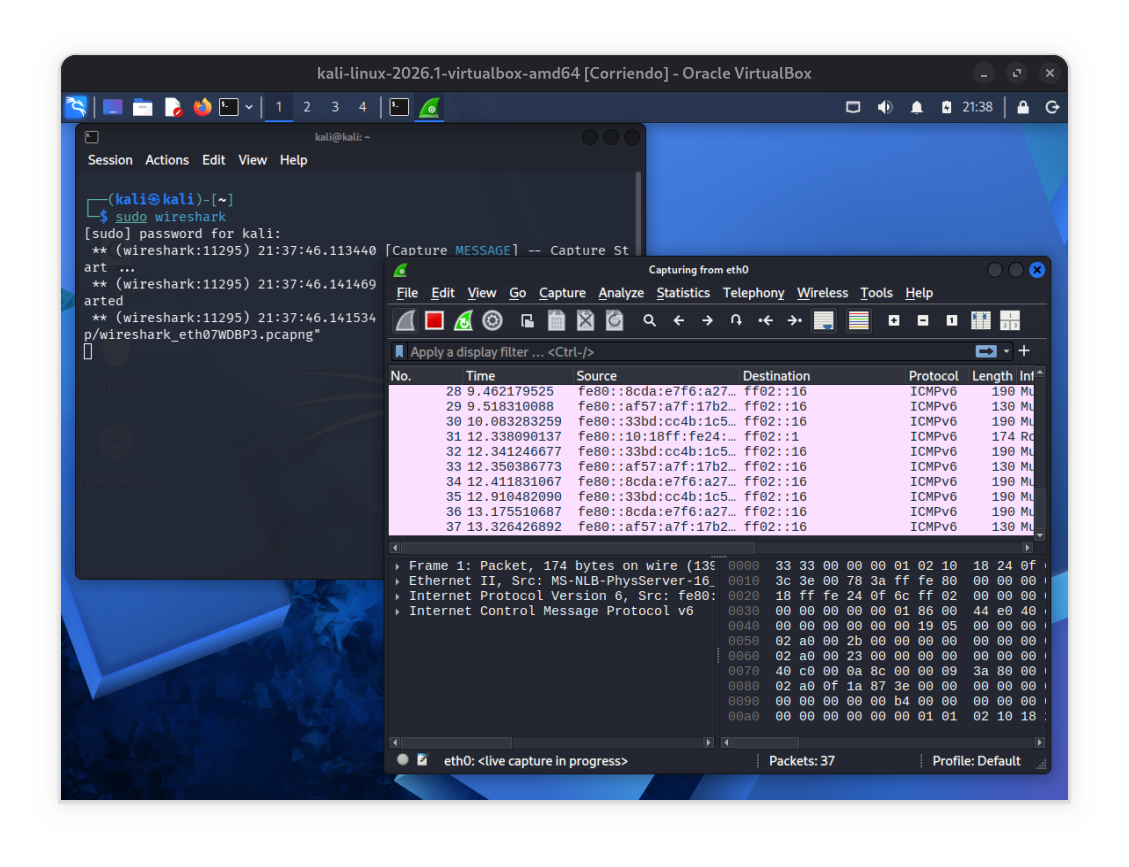
\includegraphics[scale=0.30]{imagenes/Capturas/ej-7-2.png}
	\label{fig:Ejecucion-ej-7-2}
	\vspace{-20pt}
	\caption{Wireshark en Kali Linux}
	\vspace{-20pt}
\end{figure}
Como iniciaremos con el análisis de tráfico de Telnet (en el puerto 23), aplicaremos el siguiente filtro en Wireshark: \texttt{ip.addr == 192.168.0.118 \&\& tcp.port == 23}.
\begin{figure}[H]
	\centering
	\vspace{-10pt}
	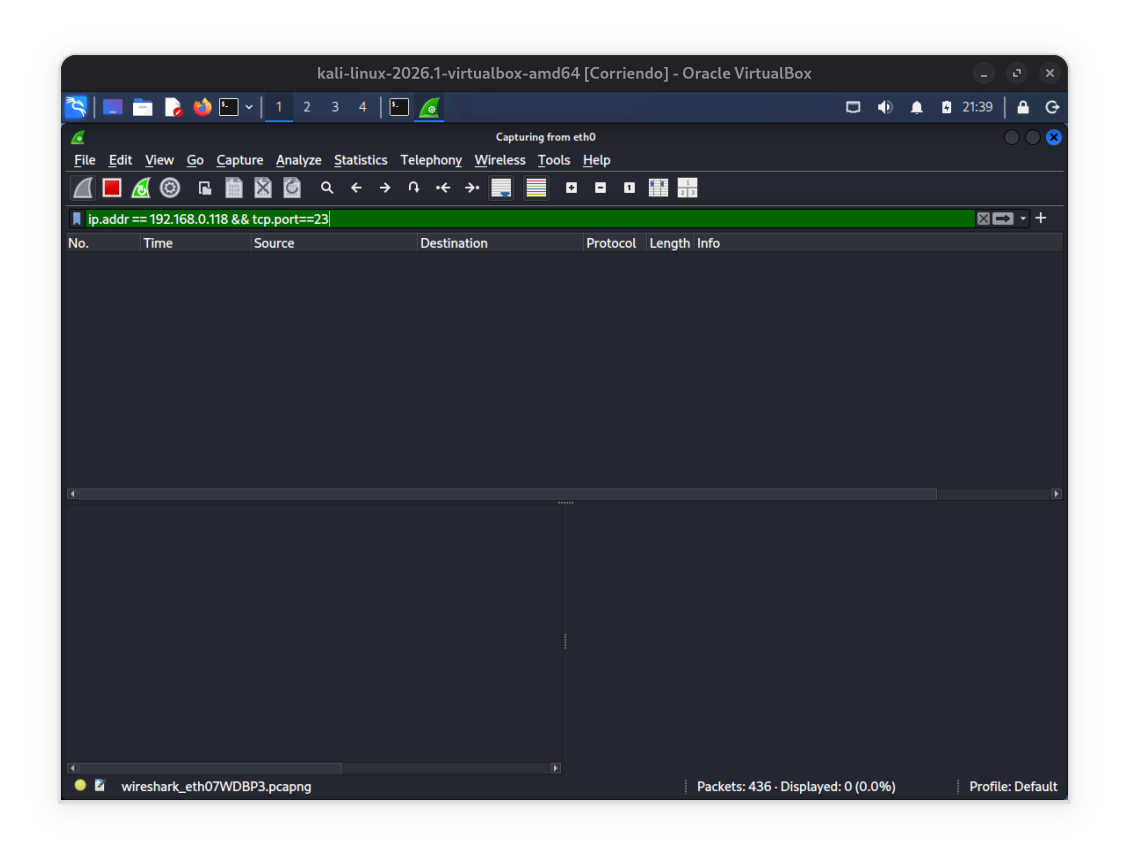
\includegraphics[scale=0.30]{imagenes/Capturas/ej-7-3.png}
	\label{fig:Ejecucion-ej-7-3}
	\vspace{-20pt}
	\caption{Filtro para Telnet en Wireshark}
	\vspace{-20pt}
\end{figure}
Con el servidor preparado, desde la máquina atacante (Kali Linux), se inició una sesión remota en otra terminal mediante el comando \texttt{telnet 192.168.0.118}, autenticándose con las credenciales del sistema y ejecutando comandos básicos como \texttt{ls} y \texttt{uname -a}. Simultáneamente, se capturaba el tráfico con Wireshark.
\begin{figure}[H]
	\centering
	\vspace{-10pt}
	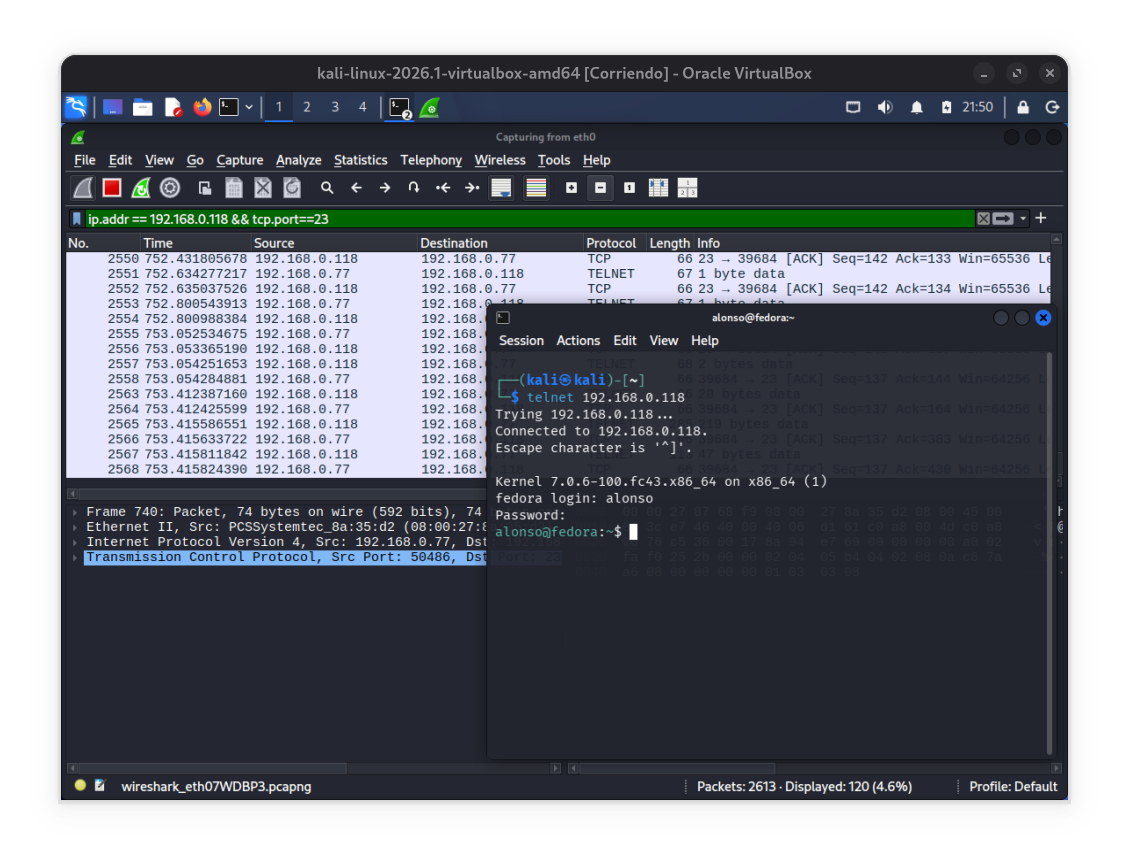
\includegraphics[scale=0.30]{imagenes/Capturas/ej-7-4.png}
	\label{fig:Ejecucion-ej-7-4}
	\vspace{-20pt}
	\caption{Conexión remota a la victima con Telnet}
	\vspace{-20pt}
\end{figure}
Posterior a esto, seleccionamos uno de los paquetes realizados con Telnet y realizamos lo siguiente para visualizar el flujo de comunicación: \textit{Click derecho} $\rightarrow$ \textit{Follow} $\rightarrow$ \textit{TCP Stream}
\begin{figure}[H]
	\centering
	\vspace{-10pt}
	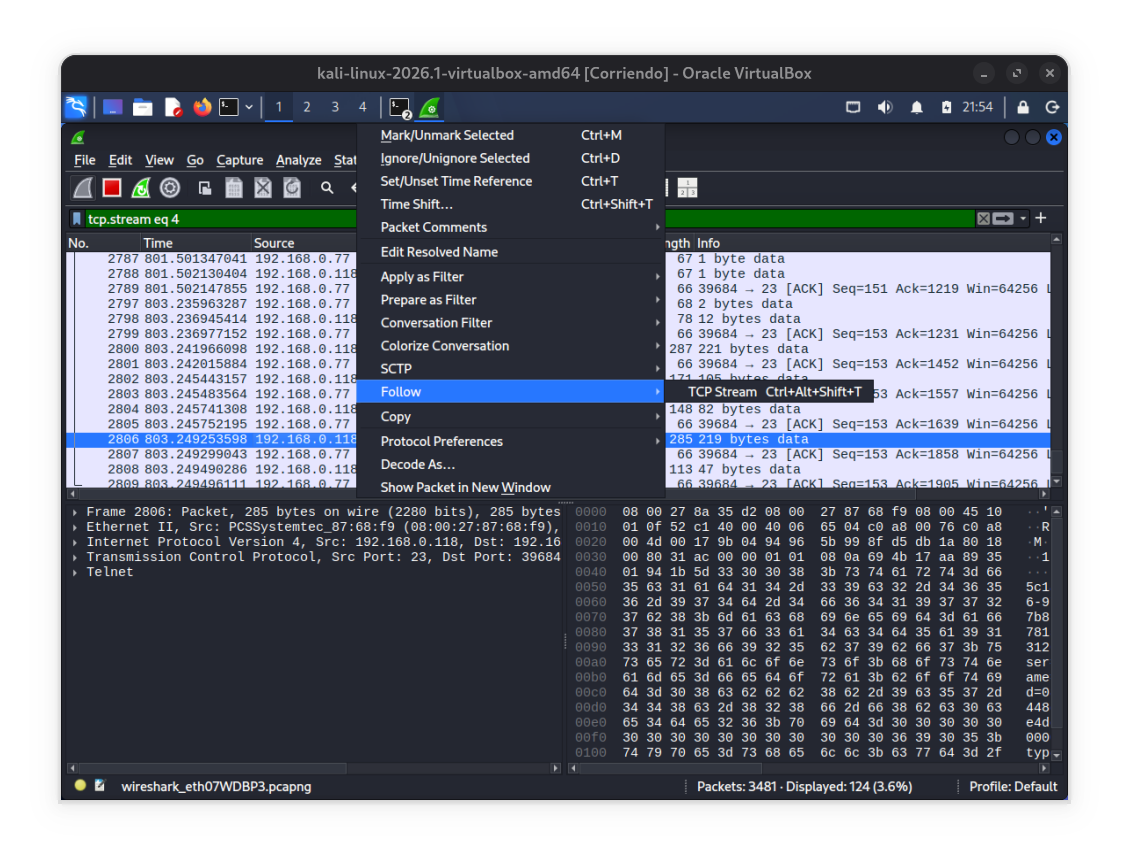
\includegraphics[scale=0.30]{imagenes/Capturas/ej-7-5.png}
	\label{fig:Ejecucion-ej-7-5}
	\vspace{-20pt}
	\caption{Pasos para la visualización del flujo TCP}
\end{figure}
\begin{figure}[H]
	\centering
	\vspace{-10pt}
	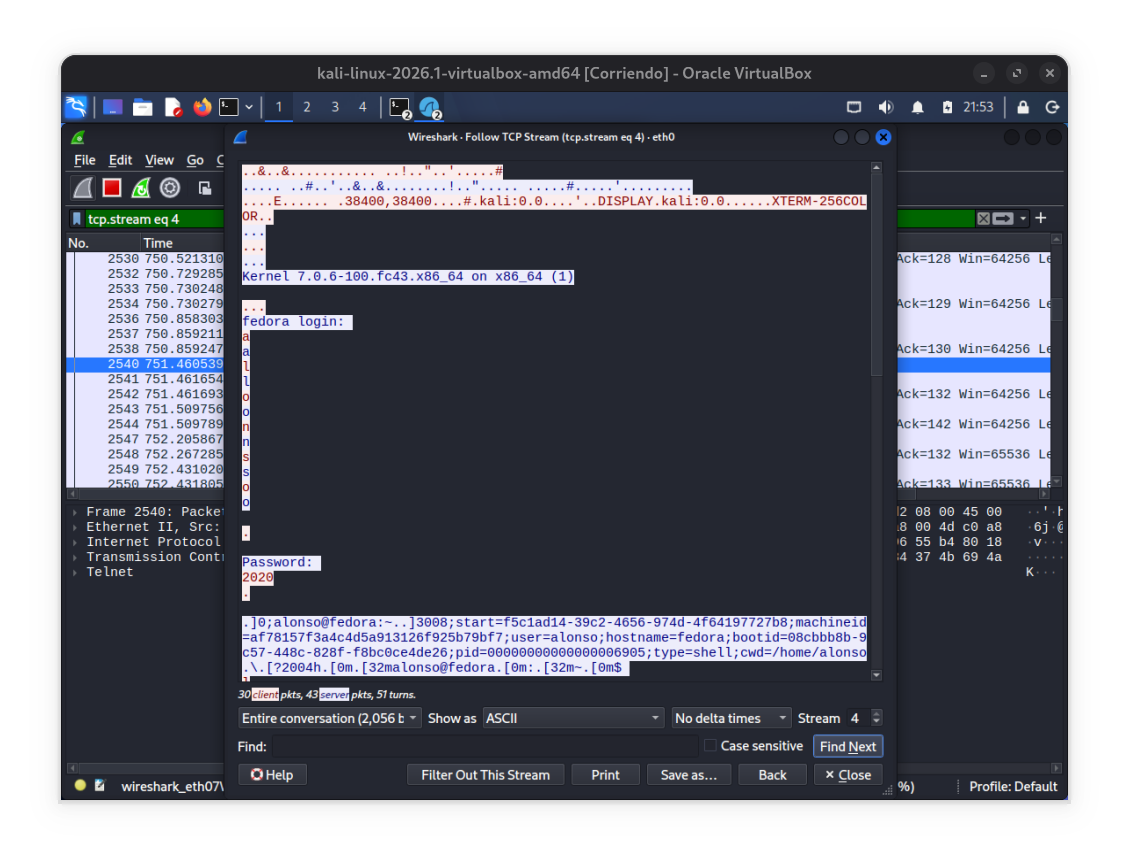
\includegraphics[scale=0.30]{imagenes/Capturas/ej-7-6.png}
	\label{fig:Ejecucion-ej-7-6}
	\vspace{-20pt}
	\caption{Visualización del usuario y contraseña en texto plano en el flujo}
\end{figure}
\begin{figure}[H]
	\centering
	\vspace{-10pt}
	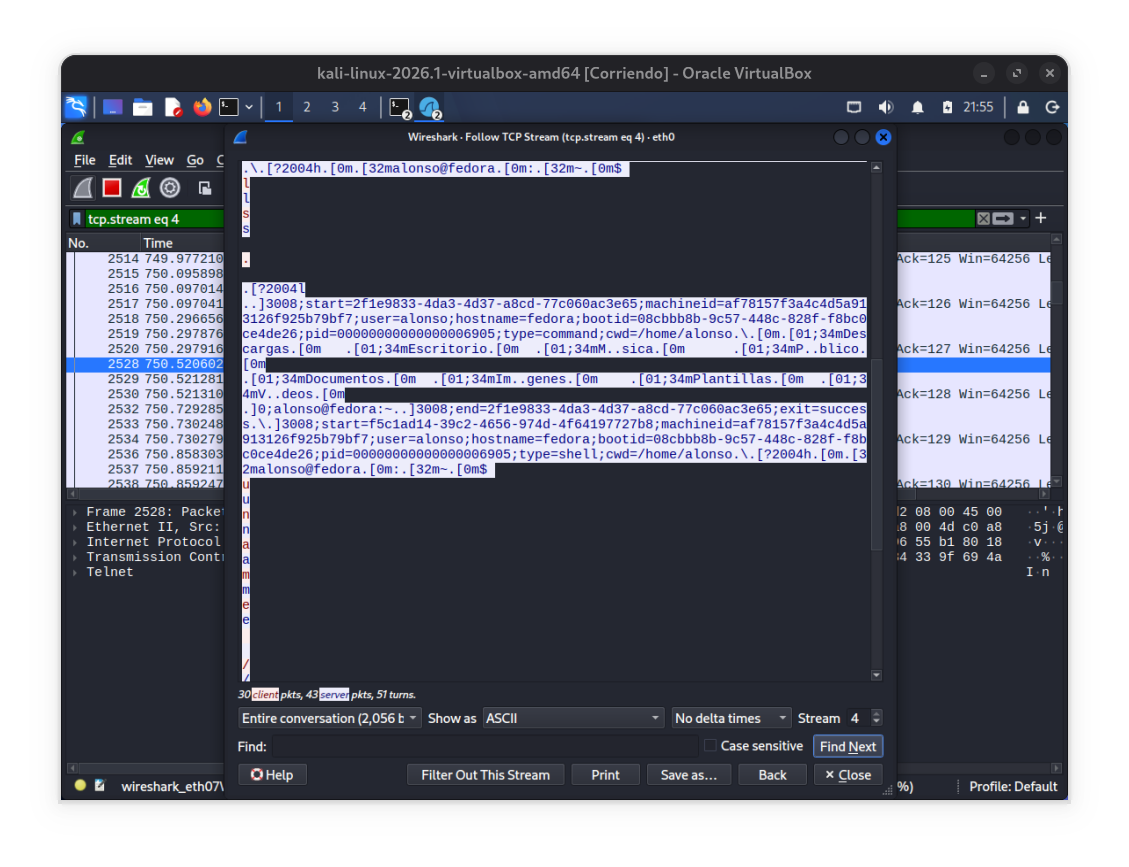
\includegraphics[scale=0.30]{imagenes/Capturas/ej-7-7.png}
	\label{fig:Ejecucion-ej-7-7}
	\vspace{-20pt}
	\caption{Visualización de comandos ejecutados en texto plano en el flujo}
	\vspace{-20pt}
\end{figure}
Al seguir el flujo TCP (TCP Stream) en Wireshark, se hace evidente la principal debilidad de Telnet: la ausencia total de cifrado. e pudo extraer absolutamente toda la interacción de la sesión en texto plano: mensajes del servidor, el nombre de usuario, la contraseña, los comandos ejecutados. \\

Después de esto se repite el experimento pero cambiando el protocolo a SSH (puerto 22). Por lo tanto preparamos Wireshark con un nuevo filtro: \texttt{ip.addr == 192.168.0.118 \&\& tcp.port == 22}.
\begin{figure}[H]
	\centering
	\vspace{-10pt}
	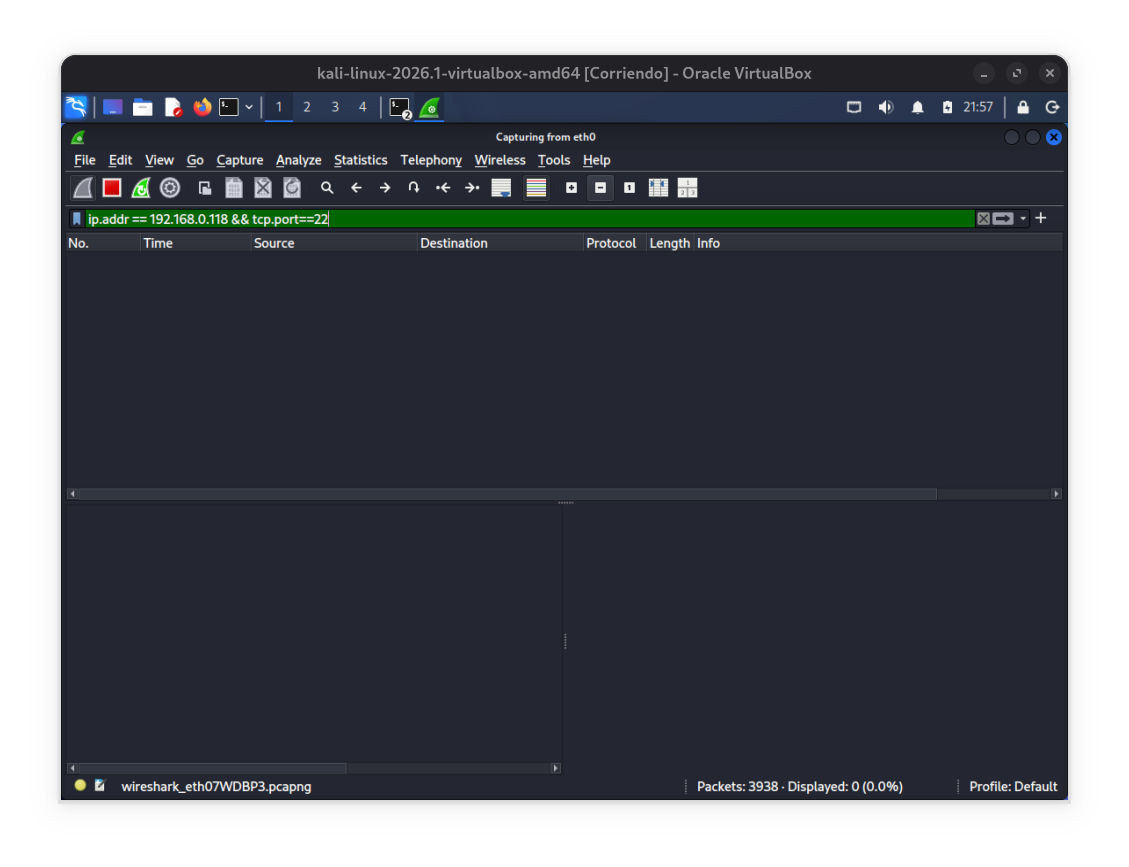
\includegraphics[scale=0.30]{imagenes/Capturas/ej-7-8.png}
	\label{fig:Ejecucion-ej-7-8}
	\vspace{-20pt}
	\caption{Filtro para SSH en Wireshark}
	\vspace{-20pt}
\end{figure}
Realizamos una nueva conexión remota usando SSH: \texttt{ssh alonso@192.168.0.118}.
\begin{figure}[H]
	\centering
	\vspace{-10pt}
	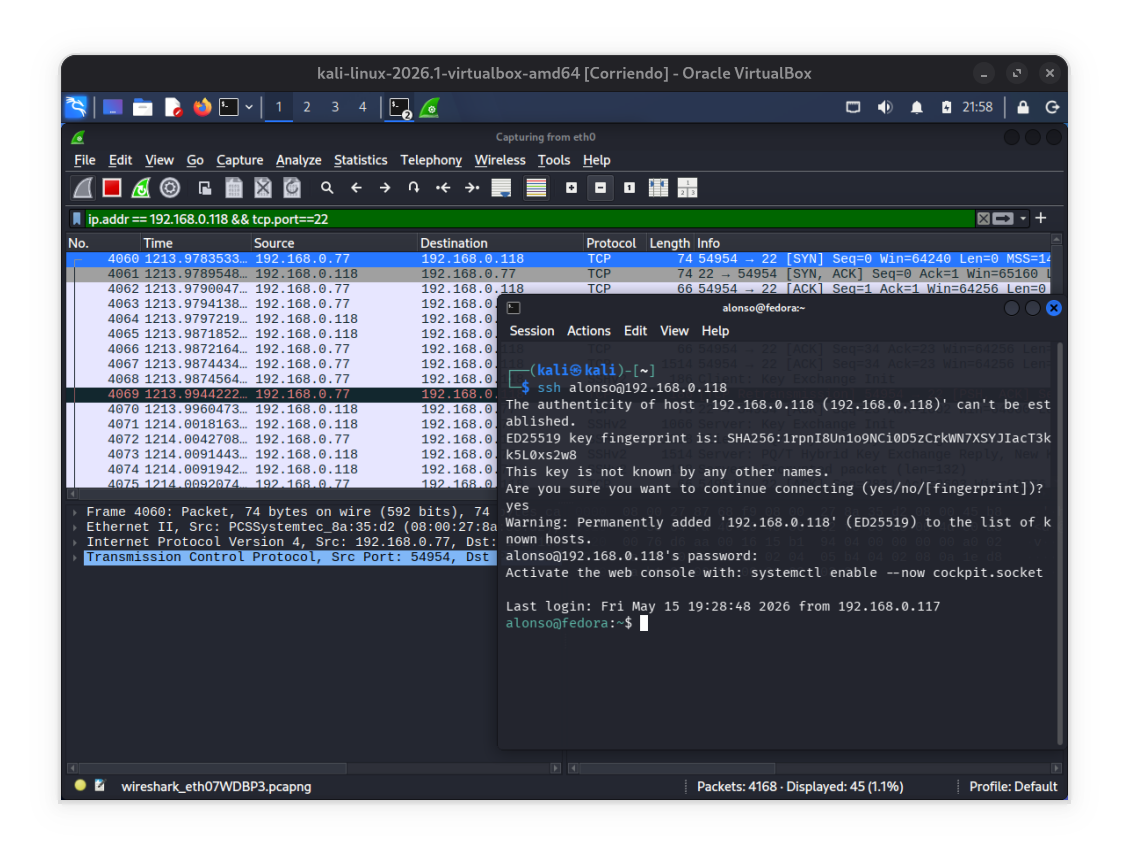
\includegraphics[scale=0.30]{imagenes/Capturas/ej-7-9.png}
	\label{fig:Ejecucion-ej-7-9}
	\vspace{-20pt}
	\caption{Conexión remota a la victima con SSH}
	\vspace{-20pt}
\end{figure}
Posteriormente, seleccionamos cualquier paquete (ahora con protocolos SSHv2) y seguimos los mismos pasos para visualizar el flujo TCP.
\begin{figure}[H]
	\centering
	\vspace{-10pt}
	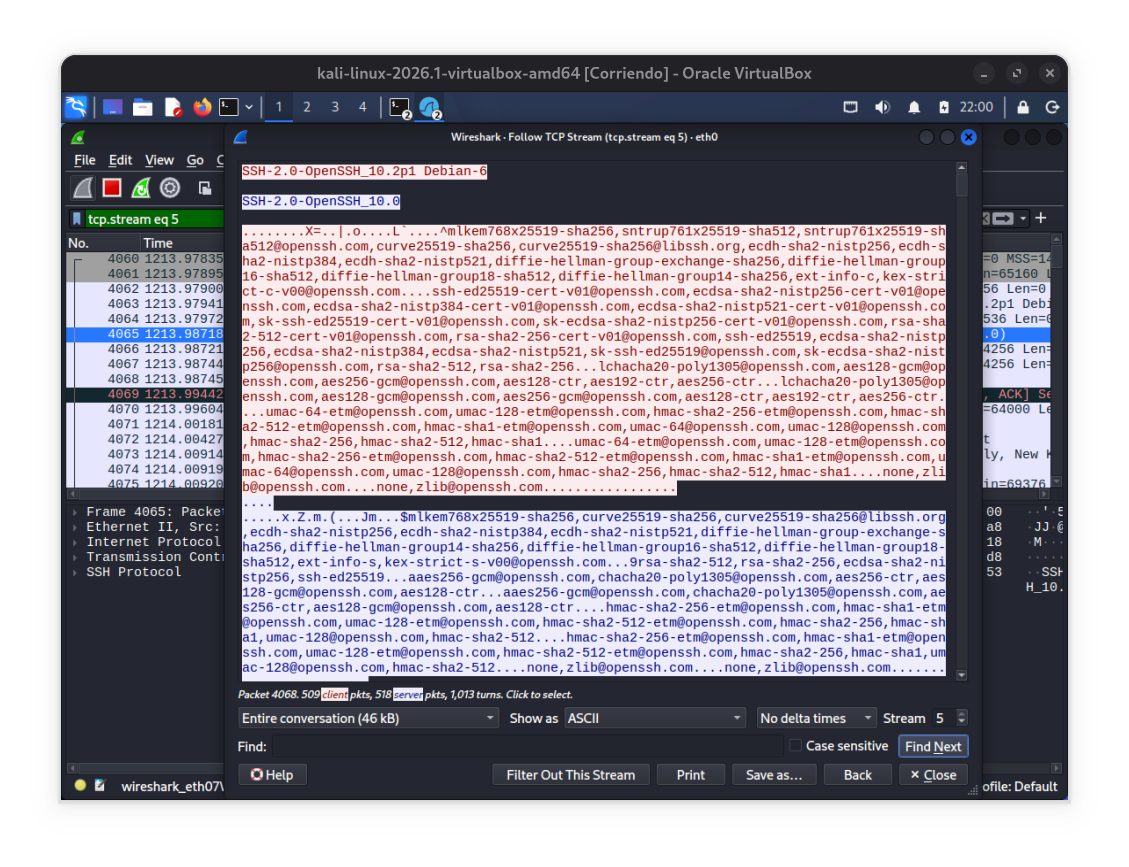
\includegraphics[scale=0.30]{imagenes/Capturas/ej-7-11.png}
	\label{fig:Ejecucion-ej-7-11}
	\vspace{-20pt}
	\caption{Visualización de comunicación cifrada en el flujo}
	\vspace{-20pt}
\end{figure}
Al abrir el flujo TCP de la captura de SSH, las primeras líneas muestran el intercambio de versiones y luego, varios algoritmos de cifrado y hasheo en texto claro. Sin embargo, después de lo anterior, todo el contenido de la pantalla se convierte en caracteres ilegibles. Es claro, que a diferencia de Telnet, el tráfico de SSH está robustamente cifrado. Es criptográficamente inviable para un atacante extraer el nombre de usuario, la contraseña, o los comandos ejecutados durante la sesión a partir de este flujo de datos interceptado.

Podemos conlcuir las razones de las porque Telnet es obsoleto y está en desuso en entornos modernos. Cualquier atacante en la red local con técnicas especializadas, puede comprometer un servidor inmediatamente si se usa Telnet. SSH soluciona esta vulnerabilidad estableciendo un túnel criptográfico seguro, garantizando la confidencialidad e integridad de la conexión remota.